% $Id: modelsandlogics.tex,v 1.3 1997/11/06 01:12:44 davek Exp davek $
\chapter{Models, Specifications and Correctness}\label{chap:methods}
\section{Introduction}\label{sec:mscintro}
Very simply, the use of formal methods in the development of a
computing system involves: 
\begin{enumerate}
\item the construction of a symbolic representation of (part of) the system,
  which captures what are believed to be essential features of its
  structure or behaviour. We call this symbolic representation \emph{a model}.
\item the construction of a symbolic representation of some desired property 
  of the system's structure or behaviour. We call this symbolic
  representation \emph{a specification}.
\item the demonstration that the property described by a specification
  is exhibited by a model of the system. Such a demonstration is said
  to establish the \emph{correctness} of the model with respect to its 
  specification. 
\end{enumerate}
There is a wide variety of languages for expressing models and specifications,
and of methods for establishing correctness. In this chapter, we 
introduce in some detail those languages and methods which are relied upon
later in the dissertation. We also give a brief review of alternatives.

Most models of real-time systems, and specifications of their
properties, employ a representation of Time. The representation which
we use is introduced in~\Sec\ref{sec:msctime}.  In \Sec\ref{sec:msclts},
we introduce \emph{labelled transition systems} and their
\emph{executions}, which serve as a unifying model of computation for
both system models and specifications. Labelled transition systems can
be described using several languages, including \emph{process algebra}
and \emph{automata} which are the topics of~\Sec\ref{sec:msctpa} and
\Sec\ref{sec:mscta}, respectively. Specifications can also be given
as automata, but in addition we use \emph{temporal logic}; these approaches
are discussed in \Sec\ref{sec:mscspec}. Verification is the topic of 
\Sec\ref{sec:mscverif}. Finally, in~\Sec\ref{sec:mscconc} we summarise
and mention briefly some other approaches to modelling, specification
and verification which have appeared in the literature.

\section{Models of Time \label{sec:msctime}}
\begin{notation}
In this section, and throughout the dissertation, the following notation is
used to denote sets of numbers: $\Time$ -- the set of non-negative real
numbers; $\rat$ -- the set of rational numbers; $\num$ -- the set of integers;
and $\nat$ -- the set of natural numbers.
\end{notation}
The model of time used in this work is the non-negative reals, which
we denote by $\Time$ and use with the usual operations of equality
($=$), ordering ($\leq$), addition ($+$), and multiplication
($\cdot$). As usual, we write $\ti < \ti'$ if $\ti \leq \ti'$ and $\ti
\neq \ti'$.  It is sometimes convenient to augment this domain with a
value, $\infinity$, which is defined to be strictly greater than any
other time value.  We write $\TimeInf$ for $\Time
\cup \{\infinity\}$ and assume that the arithmetic operators and relations are
extended to $\TimeInf$ in the usual way: for every $\ti \in \Time$, $\ti <
\infinity$, and for every $\ti \in \TimeInf$, $\ti + \infinity = \infinity +
\ti = \infinity$. We also make use of an operator for subtraction, 
$\nmin : \TimeInf \cross \Time
\fun \TimeInf$, which satisfies,
\[
\ti_1 \nmin \ti_2 =
\begin{cases}
0 & \text{if } \ti_1 < \ti_2 \\
\ti & \text{if } \ti_2 \leq \ti_1 \land \ti_1 = \ti_2 + \ti.
\end{cases}
\]

This model of time is one of a number which have been proposed for use
in the analysis of real-time systems~\cite{ah:91,jos:91,koy:91,nic:92}.  We
briefly draw attention to some salient features and their relationship
to the model of computation which will be used. 

An important choice is the one between a \emph{dense} or a
\emph{discrete} time domain. In a dense domain, such as $\Time$ or $\rat$, 
any two distinct time points are separated by a set of intervening
points which are also elements of the domain. In a discrete
domain, such as $\num$, each time point has a unique
successor. Formally, $\Time$ is a dense domain since it satisfies
\begin{zed} 
(\exists t,t' \in \Time \such t < t') \land
(\forall t,t' \in \Time | t < t' \such \exists t'' \in \Time
\such t < t'' < t')
\end{zed}
whereas $\nat$ is a discrete domain since it satisfies
\begin{zed}
\forall t,t' \in \nat \such t < t' \implies (\exists t'' \in \nat \such
t < t'' \land \forall t''' \in \nat \such t < t''' \implies t'' \leq t''').
\end{zed} 
Alur~\cite{alu:91} has argued convincingly that dense time is more
appropriate in the modelling of \emph{asynchronous} systems, where an
arbitrarily small amount of time may separate event occurrences. If a
discrete domain is chosen, then continuous physical time must be
approximated by fixing a time
\emph{granularity} a priori, and no matter how fine the granularity
chosen, for some systems the discrete model is not accurate enough to
ensure that all possible erroneous behaviours will be
detected~\cite{acd:93}. This problem has been noted also by Asarin~et
al.~\cite{amp:98a} who exhibit a class of cyclic circuits as an
example. Moreover, even when it is possible to choose a sufficiently
fine granularity, it may be so fine that the size of the state space
becomes too large for verification to be feasible. A dense domain is
also more convenient when it comes to the composition of systems,
since there is no need to worry about matching the time granularities
of the components, as is the case for a discrete model. A possible
advantage of the discrete model is that it facilitates the application
of efficient verification techniques known from the analysis of
untimed systems, in particular symbolic state space representation
using binary decision diagrams (BDDs)~\cite{bry:86,mcm:92}. It remains
to be seen whether or not efficient symbolic representations will be
discovered for dense time systems; the clock difference diagrams
of~\cite{lwy:98} show some promise in this respect. Another
interesting approach is to consider when it is possible to construct a
discrete time model which is known to preserve dense time properties,
since then we can have the expressiveness of the dense time model
together with the efficient analysis of the discrete
model~\cite{abk:97,amp:98a,bmp:97,hmp:92}.

An alternative to a \emph{point-based} domain, such as $\Time$, is a
domain based on \emph{intervals}, in which statements concerning the
duration of events may be more conveniently expressed,
see~\cite{koy:91} for further details.  In its favour, we find that
the domain $\Time$ fits naturally with a simple computational model of
time-stamped event sequences or trees.  In this model, events are
assumed to happen instantaneously, and system behaviour consists in a
sequence of \emph{two-phase steps}. In the first phase of a step, time
passes by some finite or infinite amount. In the second phase, a
finite, though arbitrarily large, number of instantaneous events occur
in some well-defined order. A new step begins when the second phase
terminates.  This two-phase model has proven very effective in
practice and is widely used; further arguments in its defence can be
found in~\cite{ns:91}. In this approach, a duration can be modelled by
introducing instantaneous events representing its beginning and end.

It is convenient to assume that event sequences respect a \emph{weakly
monotonic} ordering, i.e., for a sequence $\langle(e_1,t_1),
(e_2,t_2),\ldots\rangle$, where $e_i$ represents an event and $t_i$
its time-stamp, then $t_i$ is required to be
\emph{less than or equal to} $t_{i+1}$, rather than \emph{strictly
less than}, as would be required by a \emph{strongly monotonic}
ordering. This allows concurrency to be modelled by the interleaving
of events: for example, a computation in which the events $a$ and $b$
occur concurrently, can be modelled by the pair of sequences
$\langle\ldots, (a, t_i), (b,t_{i+1}),\ldots\rangle$ and
$\langle\ldots, (b,t_i), (a,t_{i+1}),\ldots\rangle$, where $t_i =
t_{i+1}$ in each case.  

One further point about the structure of time, which is also
intimately related to the underlying computational model, concerns
views of time as either a \emph{linear} or a \emph{branching}
structure~\cite{eh:86,lam:80,pnu:85}. In the linear model of time, it
is assumed that at any moment there is only one possible next moment;
system behaviour is represented as a set of possible execution
sequences. In the branching model, time has a tree-like structure
where it is assumed that each moment has at most one directly
preceding moment, but perhaps many next moments,
representing different possible futures; system behaviour is
represented as a tree and an execution is a path through the
tree. Each view supports the statement of system properties which
cannot be expressed in the other. We regard the two views as
complementary and make no commitment to either, but use whichever
seems appropriate in the circumstances.
   
\section{Transition Systems} \label{sec:msclts}
\subsection{Labelled Transition Systems}
A method of modelling systems and their behaviour, which has been
successfully applied in a wide variety of circumstances, is based on
the idea that it is possible to identify a set of \emph{states} which
characterise certain aspects of the system which are of interest to
the modeller. A system begins its operation in some \emph{initial
state}.  During the operation of the system, its state may change.  A
change of state is called a \emph{transition} and a system model
consisting of states and transitions is a
\emph{state transition system} (usually abbreviated to
\emph{transition system}). It is often useful to associate a
\emph{label} with a transition. The label can be used for a variety of
purposes: perhaps to identify an \emph{action} which has caused the
transition, or an \emph{event} whose occurrence is indicated by
the transition. A transition system in which labels are
associated with transitions is called a \emph{labelled transition
system} (LTS). Within this basic framework, a system modeller has wide
discretion in the choice of states, transitions and labels in the
construction of a useful model. These ideas are presented formally below.

\begin{definition}[Labelled Transition System]\label{def:msclts}
A \emph{labelled transition system} $\SS = $ 
$(\States,\Init,\Labels,{}\goes{}{})$ is a tuple where $\States$ is the set 
of states, $\Init \in \States$ is the initial state, $\Labels$ is the set 
of labels and $\goes{}\subseteq\States \cross \Labels \cross \States$ is the 
set of transitions.
\qed
\end{definition}

\begin{notation}
We write $\state \goes{\any} \state'$ for $(\state,\any,\state') \in
{}\goes{}$.  If $\state \goes{\any} \state'$ for some label $\any \in
\Labels$ then $\state'$ is said to be a $\any$\emph{-successor} of
$\state$ and $\state$ is a $\any$\emph{-predecessor} of $\state'$. If
$\state'$ is a $\any$-successor (resp. -predecessor) of $\state$, then
$\state'$ is a \emph{successor} (resp. \emph{predecessor}) of
$\state$.  If $\state$ has a $\any$-successor, we note this by $\state
\goes{\any}{}$.  If $\state$ has no $\any$-successor, we write $\state
\goesnot{\any}$. We use $\state_0 \ngoes{n} \state_n$ to denote
$\state_0 \goes{\any_0} \state_1 \goes{\any_1} \cdots \goes{\any_{n-2}}
\state_{n-1} \goes{\any_{n-1}} \state_n$, for $0 \leq i < n$ and $\any_i 
\in \Labels$, and $\state_0 \ngoes{\star} \state_f$ if $\state_0 \ngoes{n} 
\state_f$ for some $n \in \nat$.
\end{notation}

\begin{definition}[Finite, Finitely Branching, Deterministic]
A transition system, $\SS = (\States,\Init,\Labels,\TRel)$, is
\emph{finite} if the set of states $\States$ and the transition
relation $\TRel$ are finite. $\SS$ is \emph{finitely branching} if for
all $\state \in \States$ and $\any \in \Labels$, the set
$\{(\any,\state') | \state
\goes{\any} \state'\}$ is finite.  $\SS$ is \emph{deterministic} if,
for any state $\state$ and label $\any$, if $\state \goes{\any}
\state'$ and $\state \goes{\any} \state''$ then $\state' = \state''$.
\qed
\end{definition}

\begin{definition}[Isomorphism]\label{def:msciso} \mbox{\strut} \\
Let $\SS_1 = (\States_1,\Init_1,\Labels,\TRel_1)$ and $\SS_2 = (\States_2,\Init_2,\Labels,\TRel_2)$ be transition systems. $\SS_1$ and $\SS_2$ are said
to be \emph{isomorphic} iff there exists a bijection 
$f : \States_1 \fun \States_2$ such that
\begin{enumerate}
\item $f(\Init_1) = \Init_2$, and
\item for every $\state, \state' \in \States_1, \any \in \Labels$,
$\state \lgoes{1}{\any} \state'$ iff $f(\state) \lgoes{2}{\any} f(\state')$
\qed
\end{enumerate}
\end{definition}

\begin{definition}[Path]\label{def:mscpath}
Let $\SS = (\States,\Init,\Labels,\TRel)$ be a transition system.  Let
$\state \in \States$. A \emph{path} in $\SS$ \emph{from} $\state$ is a
finite or infinite sequence, $\path =
\state_0\any_0\state_1\any_1\state_2\any_2\cdots$, of alternating
states and labels which satisfies 
\begin{enumerate}
\item $\path$ starts with state $\state = \state_0$, known as the \emph{source}
  of $\path$, and
\item for all $i = 0,1,\ldots$, $\state_{i+1}$ is a $\any_i$-successor of 
$\state_{i}$. 
\qed 
\end{enumerate}
\end{definition}
A path of \emph{length} $n$ is a finite path $\path =
\state_0\any_0\state_1\any_1\cdots\any_{n-1}\state_n$. Let $\path =
\state_0\any_0\state_1\any_1\cdots$ be a finite or infinite path. For
$i = 0,1,2,\ldots$, the $i$\emph{-th state} of $\path$, denoted $\path(i)$, is
defined to be $\state_i$ and the $i$\emph{-th
label} of $\path$, denoted $\lbl{\path}(i)$, is defined to be $\any_i$.

\begin{definition}[Reachability]\label{def:mscreach}
A  state $\state'$ is
\emph{reachable} from state $\state$ iff there is a path in $\SS$ from
$\state$ which contains $\state'$.  The state $\state$ is \emph{reachable
in} $\SS$ iff $\state$ is reachable from the initial state, $\Init$.
\qed
\end{definition}

\subsection{Timed Transition Systems}\label{ss:msctts}
A real-time system can be modelled as a labelled transition
system. The actions of the system are represented by transitions whose
labels are drawn from some set $\Actions$ of actions. Such transitions
are known as \emph{discrete transitions} and are assumed to be atomic
and instantaneous.  The passage of time is modelled by transitions
whose labels are drawn from the set of non-negative real numbers
$\Time$; these transitions are called \emph{time transitions}. The set
of labels is thus $\Actions \cup \Time$. We assume $\Actions
\cap \Time =
\emptyset$.  In order to serve as a model of a real-time system, we
require that the transition system $\SS =
(\States,\Init,\Labels,\TRel)$ satisfies the following properties:
\begin{description}
\item[Time determinism] The evolution of the system is 
\emph{deterministic}
with respect to the passage of time~\cite{ns:91,nic:92,wan:90}, i.e., for a
given state and a given time, there is at most one state which can be reached
in a single step by taking the time transition.  Formally,
\[
\forall \state,\state',\state'' \in \States; t \in \Time \such
  \state \goes{t} \state' \land \state \goes{t} \state'' \implies
  \state' = \state''
\] 
\item[Time additivity] The evolution of the system is
\emph{continuous} with respect to the passage of
time~\cite{ns:91,nic:92,wan:90}. If a time transition
is possible from some state, then all smaller time transitions are also
possible. Formally,
\[
\forall \state,\state'\in \States;t,t' \in \Time \such
\state \goes{t+t'} \state' \iff
\exists \state'' \in \States \such \state \goes{t} \state''
\land \state'' \goes{t'} \state' 
\] 
\end{description}
\begin{definition}[Timed Transition System]\label{def:msctts}
A \emph{timed transition system} $\SS = (\States,\Init,\Labels,\TRel)$ is a
labelled transition system whose set of labels $\Labels$ is $\Actions \cup
\Time$ for some set $\Actions$ such that $\Actions \cap \Time = \emptyset$, 
and which satisfies the properties of time determinism and time additivity.
\qed
\end{definition}

\begin{definition}[Execution, Run]
An \emph{execution} or \emph{run} of a timed transition system $\SS$,
starting from a state $\state$, is an infinite path in $\SS$ from
$\state$. We denote the set of all executions from $\state$ by
$\Exec_{\SS}(\state)$, and by $\Exec_{\SS} = \bigcup_{\state \in
\States} \Exec_{\SS}(\state)$ the set of executions of $\SS$.  
\qed
\end{definition}

We are primarily interested in those runs which can be regarded as a
model of some physical system. In particular, we wish to ensure that
basic physical laws concerning Time are respected:
\begin{enumerate}
\item a system cannot act with infinite speed, and 
\item a system cannot block the progress of Time.
\end{enumerate}
These ideas are captured for a timed transition system in the
definition of a \emph{time-divergent} run.

\begin{definition}[Time-divergent run, Non-Zeno system]\label{def:mscdiv}
\mbox{\strut} \\ 
Let $\SS = (\States,\Init,\Labels,\TRel)$ be a timed transition
system, $\exec \in \Exec_\SS$ an execution in $\SS$ and $i, n \in
\nat$.  The $i$\emph{-th delay} in $\exec$, denoted
$\delay{\exec}(i)$, is defined to be $\lbl{\exec}(i)$ if
$\lbl{\exec}(i) \in \Time$, otherwise $\delay{\exec}(i)$ is 0. The
\emph{time elapsed} in $\exec$ from $\exec(0)$ to $\exec(n)$, denoted
$\Delay{\exec}(n)$, is defined
\[
\Delay{\exec}(n) = \sum_{i < n} \delay{\exec}(i)
\]
A run $\exec$ is \emph{time-divergent} (or simply \emph{divergent}) iff
$\lim_{i\rightarrow\infinity} \Delay{\exec}(i) = \infinity$. The set of
time-divergent runs from $\state \in \States$ is denoted 
$\Execdiv_\SS(\state)$ and the set 
$\bigcup_{\state \in \States} \Execdiv_\SS(\state)$ of all time-divergent
runs in $\SS$ is denoted $\Execdiv_\SS$.

$\SS$ is a \emph{Non-Zeno} (\emph{well-timed}) system iff every
reachable state $\state \in \States$ is the source of some
time-divergent run.
\qed
\end{definition}

\begin{remark}[Finite Variability, Time Progress]\label{rem:fvar}
It follows directly from Definition~\ref{def:mscdiv} that there are a
finite number of transitions represented in any bounded time interval
of a divergent run, $\exec$. It is also apparent that for any $t \in
\Time$, there is a number $n \in \nat$ such that $\Delay{\exec}(n) > t$, i.e.,
time progresses beyond any bound.
\end{remark}

\subsection{Composition of transition systems}\label{ss:mscltscomposition}
A complex system can be modelled by identifying and modelling smaller
components of the whole system and then by stating precisely what is the
behaviour of the system which is obtained by combining components.

A standard form of combination for transition systems is a
\emph{product} which models the parallel execution of two or more
transition systems as a single system.  We now define a commonly used
product of transition systems.  Let $\SS_1 =
(\States_1,\Init_1,\Labels_1,\TRel_1)$ and $\SS_2 =
(\States_2,\Init_2,\Labels_2,\TRel_2)$ be two transition systems which
we assume to represent system components.  In the product of $\SS_1$ and
$\SS_2$, a state is a pair $(\state_1,\state_2)$ where $\state_1\in\States_1$
and $\state_2\in\States_2$. The transitions of the product take their labels
from the set $\Labels_1 \cup \Labels_2$. If $\any$ is
a label which occurs \emph{both} in $\Labels_1$ \emph{and} in
$\Labels_2$, then we require each of $\SS_1$ and $\SS_2$ to perform a
$\any$-labelled transition together in order for the product
to perform a $\any$-labelled transition.  If the label $\any$ occurs
in the set of labels of only one component, then that component
can perform a $\any$-labelled transition
\emph{independently} in the product. The systems are said to 
\emph{synchronise} on their shared labels, otherwise they act independently.

\begin{definition}[Product of transition systems]\label{def:msctsprod} \mbox{\strut} \\
Let $\SS_1 = (\States_1,\Init_1,\Labels_1,\TRel_1)$ and $\SS_2 =
(\States_2,\Init_2,\Labels_2,\TRel_2)$ be two transition systems.
The \emph{transition system product} of $\SS_1$ and $\SS_2$, which is written 
$\SS_1 \parallel \SS_2$, is the transition
system $(\States_1 \cross \States_2, (\Init_1,\Init_2), \Labels_1
\cup \Labels_2,\TRel)$ where $(\state_1,\state_2) \goes{\any} (\state'_1,\state'_2)$ iff
\begin{enumerate}
\item $\any \in \Labels_1 \cap \Labels_2$ and $\state_1 \lgoes{1}{\any} \state'_1$ and $\state_2 \lgoes{2}{\any}
\state'_2$, or
\item $\any \in \Labels_1 \setminus \Labels_2$ and $\state_1 \lgoes{1}{\any}
\state'_1$ and $\state'_2 = \state_2$, or
\item $\any \in \Labels_2 \setminus \Labels_1$ and $\state_2 \lgoes{2}{\any}
\state'_2$ and $\state'_1 = \state_1$.
\qed
\end{enumerate}
\end{definition}

\section{Process Algebra}\label{sec:msctpa}
\subsection{Basic concepts}
The understanding of distributed systems has been advanced
considerably by the study of \emph{process algebra}. In this approach,
a system is regarded as a process, which is constructed from smaller
processes using a set of process constructors (operators).  Some
processes are regarded as primitive -- not subject to further
investigation -- and larger processes are constructed from them using
the process operators, resulting in an algebraic structure.  Processes
are investigated by considering equivalences between them, which leads to
an equational style of reasoning. There are several different
approaches to the algebraic treatment of processes. They can be
characterised by:
\begin{itemize}
\item the choice of basic processes and process operators,
\item the methods and models used to give a meaning to processes, and
\item the notion of equivalence between processes.  
\end{itemize}
The well known process algebras CCS~\cite{mil:89}, CSP~\cite{hoa:85}
and ACP~\cite{bw:90} exemplify the main variations within each of
these categories; these references should be consulted for a thorough
introduction to the field. Here we mention some aspects which may be
helpful in understanding the rest of the dissertation.

In process algebra, system events are modelled as atomic actions. In
the family of ACP algebras, atomic actions are basic processes and act
as the constants of the algebra. There is a sequential composition
operator which models the execution of one process followed by the
execution of another process. CCS adopts a different approach in which
an atomic action $a$ is not regarded as a basic process in its own
right, but can be composed with some process $\P$ using an action
prefix operator, to yield a new process $a.\P$, which is capable of
first performing the action $a$ and then behaving as process $\P$. In
this approach, the \textbf{nil} process, which cannot perform any action,
serves as a basic process. Given the possibility for modelling very
simple systems such as these, more complex systems can be constructed
using a variety of other operators including: choice, disabling,
parallel composition and abstraction. Other features of system
behaviour can also be modelled within the process algebraic framework,
e.g., process priority, memory state and shared
resources~\cite{bv:95,lbg:94}. The formal description technique
LOTOS~\cite{lot:88} offers both a variety of useful process operators
and a data language for modelling the data values which are stored and
communicated by a system. It has been used extensively for modelling
and analysing systems of practical interest.

Currently, the predominant method for giving a meaning to the terms of
a process algebra is \emph{structural operational semantics}
(SOS)~\cite{plo:81}. SOS generates a labelled transition system, whose
states are the terms of the process algebra, and whose transitions are
obtained inductively from a set of transition rules of the form
%$\stackrel{\text{premises}}{\overline{\text{\scriptsize conclusions}}}$.
$\frac{\text{premises}}{\text{conclusions}}$. An example of a typical
transition rule is
\[
\truleUD{}{\P \goes{a} \P'}{}{\P \choice \Q \goes{a} \P'}
\] 
from which we can conclude the existence of an $a$-labelled transition
from any term of the form $\P \choice \Q$ to a term of the form $\P'$,
if we can demonstrate the existence of an $a$-labelled transition from
$\P$ to $\P'$. In general, validity of the premises of a transition
rule, under a certain substitution, implies the validity of the
conclusion of this rule under the same
substitution~\cite{afv:99}. This operational style of semantic
definition gives a meaning to a process description in terms of its
effect upon the behaviour of some abstract machine. Other semantic
approaches are the denotational method of CSP~\cite{bhr:84} and the
axiomatic method of ACP~\cite{bk:84}.

A variety of process equivalences are studied in the
literature~\cite{gla:90,gla:93}.  They range from a weak equivalence,
in which processes are equated iff they can perform the same set of
transition sequences, to a strong equivalence in which they are
equated iff their derivation trees are isomorphic. The former
equivalence may equate processes $\P$ and $\Q$ even though there are
environments in which $\P$ deadlocks while $\Q$ does not. The latter
equivalence may distinguish processes even if they can perform the
same actions in all environments. Useful equivalences are found
somewhere between these extremes. The variety of useful equivalences
is greater in settings which distinguish between a set of actions
which are \emph{observable} and a set of actions which are
\emph{hidden} or \emph{silent}~\cite{gla:93}.  The process equivalence
of most relevance to our work is based on the idea of \emph{strong
bisimulation}~\cite{mil:89} and equates processes $\P$ and $\Q$ iff
for every action $a$, every $a$-successor of $\P$ is equivalent to
some $a$-successor of $\Q$, and vice versa
(cf. \Sec\ref{ss:bcstrongequivalence}). This is generally regarded as
the strongest of the useful equivalences. To be really useful, an
equivalence should also be a \emph{congruence}, i.e., equivalent
processes should behave the same in all contexts, e.g., assume $op$ is
an arbitrary process operator and $\P$ and $\Q$ are equivalent
processes, then $op(\P_1,\ldots,\P_{i-1},\P,\P_{i+1}\ldots\P_n)$ and
$op(\P_1,\ldots,\P_{i-1},\Q,\P_{i+1}\ldots\P_n)$ should also be
equivalent processes.

\subsection{Timed Extensions}
In the process algebras considered so far, there is not the
possibility to model and reason about the quantitative aspects of the
passage of time.  This deficiency has been addressed by many
researchers and, consequently, there are now many timed process
algebras which can be used in the analysis of real-time
systems. Vereijken~\cite{ver:97} gives a very comprehensive review
which covers almost 40 different timed process algebras.  Nicollin and
Sifakis~\cite{ns:91} present a helpful unifying framework.
Corradini~et~al.~\cite{cdi:99} give a detailed study of the
relationship between four CCS-like variants. Here we aim to give just
a flavour of the main themes.

In general, timed process algebras introduce constants ranging over
some time domain, either discrete or dense, and a number of time
constraining operators, into the framework of an untimed algebra. A
typical time constraining operator is one which delays a process,
e.g., let $\ti$ be a constant of the time domain, $\ti > 0$, then the
process $(\ti).\P$ is one which behaves just like $\P$ after exactly
$\ti$ time units. Such an operator is used in Temporal
CCS~\cite{mt:90}, Timed CCS~\cite{wan:90}, Real-Time CSP~\cite{dav:93}
and Urgent LOTOS~\cite{bl:91}.  $\text{ACP}_\rho$~\cite{bb:91} adopts
a different approach in which actions are time-stamped. Time stamps
can be absolute or relative. In the absolute case, $a(\ti)$ performs
the action $a$ after $\ti$ time units following the start of the
process; in the relative case, $a[\ti]$ performs $a$ after $\ti$ time
units following the execution of the previous action. The time-stamp
operator has the effect of allowing the modelling both of delays and
also of urgent actions; a delayed action becomes urgent when the time
delay expires.  Urgency can also be modelled by the introduction of
immediate actions, which do not admit the possibility of time passing
until either they are executed or disabled. This approach is adopted
in ATP~\cite{ns:94}.  Other time constraining operators which have
appeared in several algebras, and which are of practical interest for
modelling real-time systems, are the timeout and watchdog
operators. Real-time CSP offers both operators. Each takes two process
arguments $\P$ and $\Q$ and a time parameter $\ti$. The timeout $\P
\timeout[\ti] \Q$ behaves as $\P$ if an initial action of $\P$ is
performed within time $\ti$, otherwise it behaves as $\Q$, after time
$\ti$. The watchdog $\P \transfer[\ti] \Q$ behaves as $\P$ until time
$\ti$. At time $\ti$, $\P$ is aborted and $\Q$ is started.  Similar
operators are found in other algebras, e.g. ATP. 

Schneider~\cite{sch:95} discusses the operational, denotational and
axiomatic styles of semantic definition in timed process algebras, and
surveys the associated approaches to process equivalence. The decidability of
timed bisimulation is shown in~\cite{cer:92}.

We return to some of the ideas mentioned in this section in
Chapter~\ref{chap:bcandle}, where their influence on the design of the
language which is introduced there will be evident.

\section{Timed Automata}\label{sec:mscta}
\subsection{Introduction}
One of the most successful research areas of the last few years, in
the modelling and analysis of real-time systems, features the use of
\emph{timed automata}, which were introduced in the seminal paper of Alur and
Dill~\cite{ad:90}. Early work concentrated on the theoretical aspects
of the decidability and complexity of the model-checking and
satisfiability problems for timed temporal logics such as
TCTL~\cite{acd:90,ad:94,ah:91,alu:91}. Later, attention turned to the
development of practical algorithms~\cite{hnsy:94,ypd:94}. More recently, the
application of timed automata to the modelling of industrial
problems~\cite{hsl:97,lpy:98,ty:98}, and the development of software
tools to support their analysis~\cite{bll:98,bdm:98}, have been
receiving considerable attention.

Informally, a timed automaton is a finite state automaton in which the system
states are augmented by a finite number of real-valued variables called
\emph{clocks}. All clocks are synchronised and are assumed to keep perfect 
time. Transitions between states can be constrained to occur when
the values of the clocks satisfy some specified property. On the
occurrence of a transition, one or more clocks can be reset to
zero. In this way, it is possible to model the ``real time'' of
occurrence of events and the time elapsed between events. Timed automata
are presented formally below.

\subsection{Clocks}\label{ss:mscclocks}
Let $\clocks$ be a finite set of real-valued variables called
\emph{clocks}.  A \emph{$\clocks$-valuation} (clock valuation) is a 
total function $\clkvl : \clocks \fun \Time$ which assigns to each
clock $\clock \in \clocks$ a non-negative real number
$\clkvl(\clock)$.  The set of $\clocks$-valuations is denoted
$\clkvls$. The $\clocks$-valuation which assigns $0$ to every clock in
$\clocks$ is denoted $\zclkvl$.  Let $\clkvl \in \clkvls$ and
$\someclks \subseteq \clocks$.  $\clkvl[\someclks:=0]$ denotes the
valuation $\clkvl'$ such that for all $\clock \in \clocks$,
$\clkvl'(\clock)$ is $0$ if $\clock
\in \someclks$ and is $\clkvl(\clock)$ otherwise. This models the operation of
resetting some clocks while leaving the values of the other clocks
unchanged. The elapse of time is modelled by advancing the values of
all clocks in a valuation by the same amount. Let $\clkvl
\in \clkvls$ and $t \in \Time$. $\clkvl + t$ denotes the valuation $\clkvl'$
in which $\clkvl'(\clock) = \clkvl(\clock) + t$ for all clocks $\clock
\in \clocks$. Occasionally, we will need the operation $t \cdot \clkvl$
where for $t \in \Time$ and $\clkvl \in \clkvls$, $t \cdot \clkvl$ is
the valuation $\clkvl'$ such that $\clkvl'(h) = t \cdot \clkvl(h)$,
for all $\clock \in \clocks$.


\subsection{Clock Constraints}\label{ss:mscclockconstraints}
Let $\clocks$ denote a set of clocks ranged over by $\clock, \clock'$.
An \emph{atomic constraint} on $\clocks$ is an expression of the form
$\clock \genop c$ or $\clock - \clock' \genop c$, where $\genop\; \in
\{<,\leq,\geq,>\}$ and $c \in \nat$. 
The set of \emph{clock constraints} on $\clocks$, denoted $\ClockConstraints$,
is generated by the grammar:
\begin{syntax}
\clkcond & ::= & \atomcond | \clkcond \land \clkcond | \lnot \clkcond
\end{syntax}
where $\atomcond$ is an atomic constraint.  The set of \emph{clock
zones} on $\clocks$, denoted $\ClockZones$, with $\ClockZones \subset
\ClockConstraints$, is the set of conjunctions of atomic
constraints. Let $\vexcond, \vexcond'$ range over $\ClockZones$.

The restricted grammar of clock constraints is necessary in order to
ensure that some important verification questions, such as
model-checking, remain decidable. It is possible to extend the range
of $c$ to the non-negative rational numbers $\rat^+$, but the
restriction to $\nat$ simplifies the presentation at no cost to
expressive power~\cite{ad:94}.
  
A clock valuation $\clkvl \in \clkvls$ is said to \emph{satisfy} a clock
constraint $\clkcond \in \ClockConstraints$, denoted $\clkvl \models \clkcond$,
if
\begin{center}
\begin{tabular}{>$l<$>$l<$}
\clkvl \models \clock \genop c & \text{ iff } \clkvl(\clock) \genop c \\
\clkvl  \models \clock - \clock' \genop c & \text{ iff } \clkvl(\clock) - \clkvl(\clock') \genop c \\
\clkvl \models \clkcond \land \clkcond' & \text{ iff } \clkvl \models \clkcond \text{ and } \clkvl \models \clkcond' \\
\clkvl \models \lnot \clkcond & \text{ iff } \clkvl \not\models \clkcond
\end{tabular}
\end{center}
The set of all clock valuations satisfying a clock constraint 
$\clkcond \in \ClockConstraints$ is denoted $\chset{\clkcond}$, i.e.,
$\chset{\clkcond} = \{\clkvl \in \clkvls | \clkvl \models \clkcond\}$.
  
We use $\cctrue$ to denote a clock constraint such as $\clock \geq 0$
which is satisfied by any clock valuation, and $\ccfalse$ to denote a
clock constraint such as $\clock < 0$ which is not satisfied by any
clock valuation, i.e.,  $\chset{\cctrue} = \clkvls$ and
$\chset{\ccfalse} = \emptyset$.  It is also useful to have a notation
for the clock constraint which requires that all clocks have the value
$0$, $\cczero_\clocks$ denotes such a constraint, i.e., $\cczero_\clocks \defs
\bigwedge_{\clock \in \clocks} \clock = 0$, (we will just write
$\cczero$ when $\clocks$ is clear from the context). 
 
\subsection{Syntax and informal semantics}\label{ss:msctgraphs}
We can now give a formal definition of the syntax of timed automata.
We also provide some simple examples and an informal explanation of 
semantics.

\begin{definition}[Timed Automaton]\label{def:msctg}
A \emph{timed automaton} (TA) is a tuple \\
$\AA = (\tglocs,\tgiloc,\Actions,\tgclks,\tgedges,\tginv)$ where:
\begin{itemize}
\item $\tglocs$ is a finite set of \emph{control locations}.
\item $\tgiloc \in \tglocs$ is the initial control location.
\item $\Actions$ is a finite set of action labels.
\item $\tgclks$ is a finite set of clocks.
\item $\tgedges \subseteq \tglocs \cross \ClockZones \cross \Actions 
      \cross 2^\tgclks \cross \tglocs$ is a finite set of edges.  

Each edge $\tgedge \in \tgedges$ is of the form
$(\tgloc,\tgguard,a,\someclks,\tgloc')$ where $\tgloc,\tgloc' \in
\tglocs$ are control locations, denoted $\esource(\tgedge), 
\etarget(\tgedge)$, respectively; $\tgguard \in
\ClockZones$ is a clock zone, called the \emph{guard} of $\tgedge$ and 
denoted $\eguard(\tgedge)$; $a
\in \Actions$ is an action label, denoted $\elabel(\tgedge)$ and 
$\someclks \subseteq \tgclks$ is a set of clocks to be reset,
denoted $\ereset(\tgedge)$.
\item $\tginv : \tglocs \fun \ClockZones$ is a function which 
associates a \emph{time progress} condition (or \emph{invariant}) with 
each control location. Control can remain at a location while time passes 
so long as the invariant associated with the location remains true.
\end{itemize} 
We use $\cmax(\AA,\clock)$ to denote the greatest constant to which the clock
variable $\clock$ is compared in any guard or invariant condition of $\AA$,
and $\cmax(\AA)$ to denote $\max\{\cmax(\AA,\clock) | \clock \in \clocks\}$.
\qed
\end{definition}

\begin{figure}
\begin{center}
\psfrag{h1}{$h_1$}
\includegraphics[width=.4\linewidth]{METHODS/ex1.eps}
\end{center}
\caption{A simple timed automaton\label{fig:ex1}}
\end{figure}

\begin{exampleb}
We can explain some of these details informally by reference to
Figure~\ref{fig:ex1} which shows a simple example of a TA.  The set of
control locations is $\{0,1\}$. Location 0 is assumed to be the
initial location. The set of action labels is $\{a,b\}$. The set of
clocks is $\{H1\}$.  The invariant associated with location $0$ is
$\cctrue$; this means that the system can spend an arbitrary amount of
time in location 0. In the absence of an explicit clock constraint, the
edge from 0 to 1 is assumed to have the clock constraint $\cctrue$,
and so an $a$-transition from 0 to 1 is possible at any time. If an
$a$-transition occurs, clock $H1$ is reset to 0. While in location 1,
the value of clock $H1$ shows the amount of time for which control has
been at this location. Control can remain here for no more than 2 time
units, as shown by the invariant $H1
\leq 2$, i.e., the invariant serves as a way of enforcing progress:
some transition via an outgoing edge must be taken before the location
invariant becomes false. The constraint $H1 \geq 1$ on the edge from
1 to 0 ensures that a $b$-transition cannot occur until control has
resided at location 1 for at least 1 time unit, when a $b$-transition
becomes possible, taking control back to location 0. It is assumed
that no clocks are reset by a $b$-transition (the missing reset set on
the edge from 1 to 0 is taken to be $\emptyset$). The timing
requirement expressed by this automaton is that every $a$ action is
inevitably followed by a $b$ action after a delay of 1 to 2 time units.
\qed
\end{exampleb}

\subsection{Formal Semantics}\label{ss:msctasemantics}
The semantics of the timed automaton, $\AA$, is defined by assigning
a timed transition system to it. A \emph{state} in the transition system is
a pair $(\tgloc,\clkvl)$ where $\tgloc$ is a location of $\AA$ and $\clkvl$
is a clock valuation satisfying the invariant of $\tgloc$. The initial
state consists of the initial location and the clock valuation in which
all clocks are set to 0. The transition relation ${}\TRel{}$ comprises both
\emph{discrete} transitions and \emph{time} transitions. In a discrete 
transition, the location of control may change by following an
outgoing edge. In a time transition, the location of control
remains the same while time passes; the location invariant must be
satisfied throughout the passage of time. Formally,
the semantics is defined as follows:
\begin{definition}[Timed Automaton Semantics]\label{def:msctgsem}
The semantics of the timed automaton $\AA = (\tglocs,\tgiloc,\Actions,\tgclks,\tgedges,\tginv)$ is given by the timed transition system
$\TSys{\AA} = (\States,\Init,\Labels,\TRel)$ where
\begin{itemize}
\item $\States = \{(\tgloc,\clkvl) | \tgloc \in \tglocs \land \clkvl \in  \clkvls \land \clkvl \models \tginv(\tgloc)\}$.
\item $\Init = (\tgiloc,\iclkvl)$ is the initial state.
\item $\Labels = \Actions \cup \Time$ is the set of labels.
\item $\TRel \subseteq \States \cross \Labels \cross \States$ is the 
  transition relation defined by:
\begin{itemize}
\item \emph{Discrete transitions} 
\[\tadiscrete\]
We say that $(\tgloc',\clkvl[\someclks:=0])$ is a \emph{discrete successor}
of $(\tgloc,\clkvl)$.
\item \emph{Time transitions} 
\[\tatime\]
We say that $(\tgloc,\clkvl+t)$ is a \emph{time successor} of 
$(\tgloc,\clkvl)$. 
\qed
\end{itemize}
\end{itemize}
\end{definition}

\begin{notation}
If $\state = (\tgloc,\clkvl)$, then $\state + t$
denotes the state $(\tgloc,\clkvl+t)$ and $\state[\someclks:=0]$ denotes
$(\tgloc,\clkvl[\someclks:=0])$.
\end{notation}

\begin{exampleb}
Referring again to Figure~\ref{fig:ex1}, we can see that the state
space $\States \subseteq \{0,1\} \cross (\{H1\} \fun \Time)$. The initial
state is $(0,\{H1 \mapsto 0\})$. The label set $\Labels = \{a, b\} \cup
\Time$ and some possible transitions are:
\begin{eqnarray*}
(0,\{H1 \mapsto 0\}) \goes{1.7} (0,\{H1 \mapsto 1.7\}) \goes{a} (1,\{H1 \mapsto 0\}) \goes{0.2} (1,\{H1 \mapsto 0.2\}) \goes{1.3} \\
(1,\{H1 \mapsto 1.5\}) \goes{b} (0,\{H1 \mapsto 1.5\}) \goes{50} (0,\{H1 \mapsto 51.5\}) \goes{a} (1,\{H1 \mapsto 0\}) \ldots
\end{eqnarray*}
\qed
\end{exampleb}

We define a notion of \emph{deterministic} timed automata by analogy
with the classical notion of determinism for finite state
automata, viz., the state reached by following an edge with a given
label is uniquely determined by the current state. However, in the case
of timed automata, it is not necessary to prohibit the use of the same label on
distinct outgoing edges of every location, but, instead, it is required only 
that for any pair of such edges, the associated  clock constraints are mutually
exclusive, so that at any time at most one of them is enabled.
\begin{definition}[Deterministic Timed Automaton]
A timed automaton is said to \emph{deterministic} iff for all 
$\tgloc \in \tglocs$, for all $a \in \Actions$ and for every pair of
distinct edges of the form $(\tgloc,\tgguard_1, a, \someclks_1, \tgloc')$ and 
$(\tgloc, \tgguard_2, a, \someclks_2, \tgloc'')$, there is no
clock valuation $\clkvl$ which satisfies \emph{both} of the
following conditions:
\begin{enumerate}
\item $\clkvl \models \tgguard_1$ and $\clkvl[\someclks_1:=0] \models 
  \tginv(\tgloc')$,
\item $\clkvl \models \tgguard_2$ and $\clkvl[\someclks_2:=0] \models 
  \tginv(\tgloc'')$. 
\qed
\end{enumerate}
\end{definition}


\subsection{Composition of timed automata}\label{ss:msctacomposition}
By defining a product for timed automata, we can model a complex system using
several smaller, interacting component automata.

Let $\AA_1 = (\tglocs_1, \tgiloc_1, \Actions_1, \tgclks_1, \tgedges_1, \tginv_1)$
and $\AA_2 = (\tglocs_2, \tgiloc_2, \Actions_2, \tgclks_2, \tgedges_2, \tginv_2)$
be two timed automata. Assume that the clock sets $\tgclks_1$ and $\tgclks_2$
are disjoint. Then the product, denoted $\AA_1 \parallel \AA_2$, is the timed
automaton $(\tglocs_1 \cross
\tglocs_2, (\tgiloc_1,\tgiloc_2), \Actions_1 \cup \Actions_2, \tgclks_1 \cup \tgclks_2, \tgedges, \tginv)$, where 
$\tginv(\tgloc_1,\tgloc_2)$ is defined to be $\tginv_1(\tgloc_1) \land
\tginv_2(\tgloc_2)$ and the edges $\tgedges$ are given by:
\begin{enumerate}
\item For $a \in \Actions_1 \cap \Actions_2$, for every 
$(\tgloc_1,\tgguard_1,a,\someclks_1,\tgloc'_1) \in \tgedges_1$ and $(\tgloc_2,
\tgguard_2,a,\someclks_2,\tgloc'_2) \in
\tgedges_2$, $\tgedges$ contains $((\tgloc1,\tgloc2),\tgguard_1 \land \tgguard_2,a,\someclks_1 \cup \someclks_2,(\tgloc'_1,\tgloc'_2))$
\item For $a \in \Actions_1 \setminus \Actions_2$, for every 
$(\tgloc_1,\tgguard,a,\someclks,\tgloc'_1) \in \tgedges_1$ and every 
$\tgloc_2 \in \tglocs_2$, $\tgedges$ contains
$((\tgloc_1,\tgloc_2),\tgguard,a,\someclks,(\tgloc'_1,\tgloc_2))$
\item For $a \in \Actions_2 \setminus \Actions_1$, for every
$(\tgloc_2,\tgguard,a,\someclks,\tgloc'_2) \in \tgedges_2$ and every 
$\tgloc_1 \in \tglocs_1$, $\tgedges$ contains
$((\tgloc_1,\tgloc_2),\tgguard,a,\someclks,(\tgloc_1,\tgloc'_2))$
\end{enumerate}

From this we can see that the locations of the product are just pairs of
component locations and the invariant of a compound location is the
conjunction of the invariants of its component locations. The edges are
obtained by synchronising edges with identical labels.

For timed automata $\AA_1$ and $\AA_2$, it can be shown that the
product of the models of $\AA_1$ and $\AA_2$ is the same as the model
of the product of $\AA_1$ and $\AA_2$; i.e., $\TSys{\AA_1} \parallel
\TSys{\AA_2}$ is isomorphic to $\TSys{\AA_1 \parallel
\AA_2}$~\cite{ad:94}.  Figure~\ref{fig:ex2} shows a simple example of
a product construction of timed automata.

\begin{figure}
\begin{center}
\begin{tabular}{|c|}
\hline
\multicolumn{1}{|l|}{$\AA_1$} \\
\includegraphics[width=.3\linewidth]{METHODS/a1.eps} \\
\hline
\multicolumn{1}{|l|}{$\AA_2$} \\
\includegraphics[width=.3\linewidth]{METHODS/a2.eps} \\
\hline
\multicolumn{1}{|l|}{$\AA_1 \parallel \AA_2$} \\
\includegraphics[width=.7\linewidth]{METHODS/a1compa2.eps} \\
\hline
\end{tabular}
\end{center}
\caption{Product construction for timed automata\label{fig:ex2}}
\end{figure}

\begin{exampleb}[Train Gate Controller]
The level crossing controller is a ubiquitous introductory example.
We consider a simple system consisting of three components: a train, a
gate and a controller. Each of these can be modelled as a TA (see
Figure~\ref{fig:tgc}). Timing constraints are expressed using 3
clocks: $H1$ for the train, $H2$ for the gate and $H3$ for the
controller. The train advises the controller of its approach more than
2 minutes before it enters the crossing.  The approach of the train is
indicated by the action {\tt approach}, and entry into the
crossing by the action {\tt in}. Notice that the guard on the edge
labelled {\tt in} is {\tt H1 > 2}. The maximum delay between the
actions {\tt approach} and {\tt exit} is 5 minutes. The gate is open in
location {\tt Gate.0} and closed in location {\tt Gate.2}. The actions
{\tt raise} and {\tt lower} are used to indicate requests for service
from the gate by the controller.  The actions {\tt up} (resp. {\tt
down}) indicate that the gate has been completely raised
(resp. lowered). The controller idles in location {\tt
Controller.0}. Whenever it detects that the train is approaching, it
requests that the gate should be lowered. Similarly, whenever it
detects that the train has left the crossing, it requests that the
gate should be raised. The complete system is expressed as the
composition of the three components {\tt Train | Gate | Controller}.
The safety requirement for the system is straightforward: whenever the
train is in the crossing, the gate should be closed.
\qed
\end{exampleb}

\begin{figure}
\begin{center}
\begin{tabular}{|c|}
\hline
\multicolumn{1}{|l|}{\bf Train} \\
\includegraphics[width=.75\linewidth]{METHODS/train.eps} \\
\hline
\multicolumn{1}{|l|}{\bf Gate} \\
\includegraphics[width=.75\linewidth]{METHODS/gate.eps} \\
\hline
\multicolumn{1}{|l|}{\bf Controller} \\
\includegraphics[width=.5\linewidth]{METHODS/controller.eps} \\
\hline
\end{tabular}
\end{center}
\caption{Level Crossing Control System\label{fig:tgc}}
\end{figure}

\section{Property Specification}\label{sec:mscspec}
The main point of constructing a formal system model is to check it
for the presence of desirable properties and the absence of
undesirable properties. A first step in this direction involves
formally stating the properties of interest. A classification of 
properties which has proved of enduring usefulness is the distinction
between \emph{safety} and \emph{liveness} properties,
introduced by Lamport~\cite{lam:77,lam:80}. Informally, a safety
property specifies that `nothing bad ever happens', while a
liveness property specifies that `something good eventually happens'.
There is a variety of approaches to expressing both safety and
liveness properties of timed transition system models. We consider
some of them in this section. The remainder of the section is
structured as follows.  In~\Sec\ref{ss:mscstateproperties}, we
consider the expression of properties of individual states using
\emph{state formulas}. This allows us to state simple safety
invariants which can be checked by exploring all reachable states and
testing them for satisfaction of the invariant property. More
complicated properties, involving system executions, can be expressed
using \emph{specification automata} or \emph{temporal logic}. These
approaches are considered in \Sec\ref{ss:mscautomata} and
\Sec\ref{ss:msctemporallogic}, respectively. The relationship 
between automata and temporal logic is considered 
in~\Sec\ref{ss:mscpropdiscussion}.

\subsection{State Properties}\label{ss:mscstateproperties}
For a state transition model, $\SS$, the simplest properties to assert
and check are those concerned only with individual states, i.e. given
some state $\state$ determine whether or not a property $\sfmla$ holds
at $\state$. What structure we attribute to a state will depend on the
circumstances. At the least, we assume that a state is
associated with a unique identifier;
sometimes, in addition, we assume that a state gives a valuation for a
set of typed variables. Let $\Var$ be such a set and let $\xx$ range
over $\Var$.  The value of $\xx$ at state $\state$ is denoted
$\state.\xx$. We assume that a \emph{state formula} $\sfmla$ is a boolean
expression constructed in the usual way from variables, function
symbols, predicate symbols and boolean connectives, and that there is
a valuation function $\eval{\sfmla}_\state$, which gives the value of
$\sfmla$ at $\state$. We write $\state \smodels
\sfmla$ iff $\eval{\sfmla}_\state = \true$. The reader should refer 
to~\cite{mp:92} for further explanation of state formulas, if required.

Let $\SS = \TSys{\AA}$
be a transition system, where the TA $\AA = (\tglocs, \tgiloc,
\Actions, \tgclks, \tgedges, \tginv)$ is either a simple TA, or a composition
of TA $\AA_1 \parallel \cdots \parallel \AA_n$.  Then
$\enable(a)$ and $\AA_i \at \tgloc$ can be encoded as state formulas,
where $a \in \Actions$ is an action and $\tgloc \in \tglocs$ is a
location. Informally, $\enable(a)$ is true if it is possible to take
an $a$-transition from the current state, and $\AA_i \at \tgloc$ is
true if control in the TA $\AA_i$ currently resides at location
$\tgloc$.

Formally, 
\[ (\tgloc,\clkvl) \smodels \enable(a) \text{ iff } \exists(\tgloc,\tgguard,a,\someclks,\tgloc') \in \tgedges \such \clkvl \models \tgguard \land \clkvl[\someclks := 0] \models \tginv(\tgloc')
\]
and, for $1 \leq i \leq n$,
\[ ((\tgloc_1,\tgloc_2,\ldots,\tgloc_n),\clkvl) \smodels \AA_i \at \tgloc_i.
\]

\begin{exampleb}
Let $\SS = \TSys{\mbox{\tt Train | Gate | Controller}}$, where {\tt
Train}, {\tt Gate} and {\tt Controller} are as given in
Figure~\ref{fig:tgc}.  Let $\tgloc = (1,1,0)$, i.e. $\tgloc$ is a
compound location in which the components are: {\tt Train} at location
1, {\tt Gate} at location 1 and {\tt Controller} at location 0. Let
$\clkvl = \{\clock_1 \mapsto 1.5, \clock_2 \mapsto 0.5, \clock_3
\mapsto 1.5\}$ be a clock valuation. Let $\state = (\tgloc,\clkvl)$.
Then, we have $\state \smodels \enable(down)$ and 
$\state \smodels \mbox{\tt Gate}\at 1$, but $\state \not\smodels \enable(in)$
and $\state \not\smodels \mbox{\tt Controller} \at 1$.
\qed
\end{exampleb}

\begin{exampleb}
Let $\state$ be a state over integer variables $\xx,\yy$ and 
boolean variable $\zz$, such that $\state = \{\xx \mapsto 5, \yy \mapsto 7,
\zz \mapsto \True\}$. Then, $\state \smodels \zz$, 
$\state \not\smodels \xx > \yy$, $\state \smodels \xx + \yy < 15$ and
$\state \smodels \zz \implies (\yy - \xx = 2)$.
\qed
\end{exampleb}

\begin{exampleb}
In the level crossing control system of Figure~\ref{fig:tgc},
the safety requirement can be stated as the absence of any reachable
state $\state$ satisfying $\state \smodels \mbox{\tt Train}\at 2 \land
\lnot \mbox{\tt Gate} \at 2$.
\qed
\end{exampleb}

\subsection{Automata\label{ss:mscautomata}}
We can go beyond checking simple state properties and check properties
of executions by reasoning about the system in the context of a
testing (observer) automaton. Given a TA $\AA_M$ which models the
behaviour of a system, a test TA $\AA_S$ is constructed to capture a
property specification, and the composition $\AA_M
\parallel \AA_S$ is checked to see if some error state is 
reachable. Using this technique it is possible, for example, to test a
bounded response property, i.e., that the occurrence of a stimulus is
followed by a response within a bounded period of time.

\begin{exampleb}
Figure~\ref{fig:tgcresponse}\footnote{Standard abbreviations are used
in the figure to reduce its size: an edge labelled with a set of
actions $\Actions$ represents a set of edges, one for each action in 
$\Actions$; for any action $a \in \Actions$, the notation ${}\setminus{a}$ 
stands for the set $\Actions \setminus \{a\}$.} shows a test automaton for the
level crossing control system. The test automaton is used to check the
bounded response property `the gate is always raised strictly within
10 minutes of being lowered'. We consider the behaviour of the
composition {\tt Train | Gate | Controller | Test}. A {\tt down} action
in {\tt Gate} synchronises with a {\tt down} action in {\tt Test},
causing a transition in {\tt Test} to location 1, resetting the test
clock {\tt Ht}. The invariant {\tt Ht <= 10} ensures that control can
reside at {\tt Test.1} for no more than 10 minutes.  At any time
before 10 minutes, an occurrence of any action other than {\tt up}
leaves control at {\tt Test.1}; an {\tt up} action returns control to
{\tt Test.0}.  When 10 minutes have passed at {\tt Test.1}, the only
possible action for {\tt Test} is {\tt fail}, which takes control to
the error location {\tt Test.2}. The bounded response property for the
system is satisfied iff it is not possible to reach a state satisfying
{\tt Test@2}.
\qed
\end{exampleb}

\begin{figure}
\begin{center}
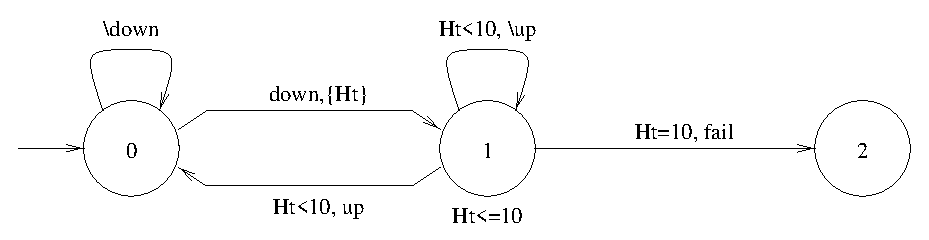
\includegraphics[width=.75\linewidth]{METHODS/tgcresponse.eps}
\end{center}
\caption{{\tt Test} automaton for bounded response\label{fig:tgcresponse}}
\end{figure}

The approach to property checking via test automata is closely related
to classical verification methods based on language
containment~\cite{ad:94,kur:94,tho:90}. We give a brief
introduction to the use of such a method for timed systems. 

Let $\AA_M$ be a TA defining a system model and $\AA_S$ a TA, extended
with an \emph{acceptance condition}, which defines a property
specification. Let $\Lmodel = \Execdiv(\Init_M)$ be the set of
non-Zeno executions of $\AA_M$ and $\Lspec = \{\exec \in
\Execdiv(\Init_S) | \exec \text{ satisfies the acceptance condition of } 
\AA_S\}$ the set of those non-Zeno executions of $\AA_S$ which satisfy 
its acceptance condition. $\Lmodel$ is called the \emph{language} of
$\AA_M$ and $\Lspec$ the language of $\AA_S$. The system model
satisfies the specification iff $\Lmodel \subseteq \Lspec$, i.e., if
the language $\Lmodel \cap \compl{\Lspec} = \emptyset$. Intuitively,
$\AA_S$ defines the set of all \emph{allowed} executions and $\AA_M$
defines the set of all \emph{possible} executions of the system. The
verification problem is to show that all possible executions are
allowed or, equivalently, that no disallowed execution is
possible. Attention is restricted to the non-Zeno executions since
they are the only ones which can reasonably be judged to model the
behaviour of a physical system.

Several acceptance conditions have been proposed in the
literature~\cite{tho:90}. For timed systems, \Buchi\ acceptance
and Muller acceptance have received most attention~\cite{ad:94}.
Here we concentrate on \Buchi\ acceptance.

\Buchi\ acceptance is defined for a TA $\AA = (\tglocs, \tgiloc, \Actions, 
\tgclks, \tgedges, \tginv)$ augmented with a set $\F \subseteq 
\tglocs$ of \emph{accepting} locations. In any execution, one or more locations
are visited infinitely often. Let $\infoften(\exec)$ be the set of all
infinitely occurring locations of the execution $\exec$. $\exec$
is \emph{accepted} iff $\infoften(\exec) \cap \F \neq \emptyset$, i.e.
if some accepting state occurs infinitely often in it. A timed automaton
extended with a \Buchi\ acceptance condition is called a timed \Buchi\
automaton (TBA). 

In practice, the test for language containment $\Lmodel\subseteq
\Lspec$ is usually implemented by constructing the automaton $\AA_M
\parallel \compl{\AA_S}$ and checking for the absence of any
acceptance cycle.  A problem with this approach is the requirement to
construct the complement $\compl{\AA_S}$ of the specification
automaton $\AA_S$, since TBA are not closed under
complementation. However, if $\AA_S$ is deterministic then it can be
complemented effectively. The restriction to deterministic TBA still
allows the expression of a wide range of specifications.  An even more
pragmatic approach to the problem of complementation is to avoid it
entirely by requiring the specifier to provide $\compl{\AA_S}$
directly, rather than $\AA_S$. This approach is adopted, for example,
in~\cite{tri:98} where an efficient algorithm is given for
testing TBA emptiness.

\begin{exampleb}
Figure~\ref{fig:tgcresponsetba}\footnote{Accepting locations are
shown as a double circle, as usual.} shows a deterministic TBA which
specifies the bounded response property for the level crossing control
system.
\qed
\end{exampleb}

\begin{figure}
\begin{center}
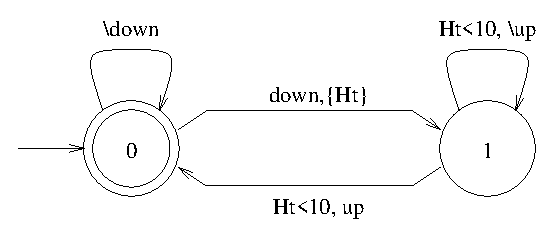
\includegraphics[width=.6\linewidth]{METHODS/tgcresponsetba.eps}
\end{center}
\caption{TBA for bounded response\label{fig:tgcresponsetba}}
\end{figure}
  
\subsection{Temporal Logic\label{ss:msctemporallogic}}
Temporal logic~\cite{eme:90} was developed originally in the field of
philosophy, where it was used to describe and reason about how the
truth values of assertions vary with time. For some assertion $\fmla$,
typical temporal operators include \emph{sometime} $\fmla$, which is
true now if $\fmla$ will become true at some time in the future, and
\emph{always} $\fmla$, which is true now if $\fmla$ is true now and
forever more. Pnueli~\cite{pnu:77} was the first to show how temporal
logic could be used to reason about the behaviour of computer
programs, particularly \emph{reactive} programs such as operating
systems and communication protocols. This early work often involved a
difficult manual construction of the proof of some program property.
Interest in the use of temporal logic for program specification
increased when it was shown that the validity of a specification for a
given program could be determined \emph{automatically} by \emph{model
checking}~\cite{ce:81,qs:81}, i.e., by checking the truth or falsehood
of the specification when interpreted using the program as a
model. The EMC model checker, developed at Carnegie Mellon, allowed
small programs to be checked automatically in linear time for
satisfaction of specifications written in the branching time logic
CTL~\cite{ces:86}. Activity in the area intensified with the
introduction of \emph{symbolic} methods~\cite{bcm:92,mcm:92} which
facilitate the storage of the large state spaces which arise in the
checking of realistic programs. The extension of temporal logics with
\emph{explicit references to time quantities} was motivated by the
desire to apply temporal logic to the specification and verification
of real-time programs, where, for example, it is not enough to assert
just ``\emph{sometime} $\fmla$'', but rather ``\emph{sometime within
the next 5 seconds} $\fmla$''. Early quantitative temporal logics were
based upon a discrete model of
time~\cite{ah:93,eme:91,ems:90,hlp:90,ost:86}.  However, the
decidability of the model-checking problem for a
\emph{dense time} model was demonstrated in~\cite{acd:90} which
introduced Timed Computation Tree Logic (TCTL), a timed extension of
CTL. The usefulness of this result was advanced by~\cite{hnsy:94}
which gave a practical method for implementing the model-checking of
timed automata with respect to TCTL specifications; this method has
been implemented in the verification tool KRONOS~\cite{bdm:98}. An
efficient, on-the-fly implementation of model-checking for \etctl, a
logic strictly more expressive than TCTL, is proposed
in~\cite{bty:97}.

It is outside the scope of this dissertation to provide a detailed
survey of temporal logics and model-checking, for which we refer the
reader to the literature~\cite{ah:91,cgp:99,eme:90,yov:97}; however, we do
provide an introduction to TCTL, since it is used in the
rest of the dissertation for specifying real-time properties.

\subsubsection{TCTL: Syntax and Semantics}
Let $\II$ denote the set of all intervals of $\Time$ of the form
$[c,c'], [c,c'), (c,c'], (c,c')$, $[c,\infinity]$ and $(c,\infinity)$
where $c,c' \in \nat$.
The set of TCTL formulas is defined by the following syntax: 
\begin{syntax}
\fmla & ::= & \sfmla | \lnot \fmla | \fmla \lor \fmla | \fmla \euntil{\I} \fmla | \fmla \auntil{\I} \fmla
\end{syntax}
where $\sfmla$ is a state formula and $\I \in \II$ is an 
interval.

Let $\AA$ be a TA. TCTL formulas are interpreted with respect to the
transition system $\TSys{\AA} = (\States,\Init,\Labels,\TRel)$, and
a satisfaction relation $\smodels$ for state formulas $\sfmla$. The
fact that a state $\state
\in \States$ satisfies a TCTL formula $\fmla$ is denoted 
$\state \models_{(\AA,\smodels)} \fmla$ (the subscript is usually
omitted to avoid clutter). The dense nature of the time model requires
us to take some care in the definition of satisfaction for TCTL and it
is helpful to introduce some further notation before giving a formal
definition. For a state $\state$, the temporal modalities
$\euntil{\I}$ and $\auntil{\I}$ are interpreted with respect to the
non-Zeno executions starting from $\state$, i.e.,
$\Execdiv_{\AA}(\state)$. Suppose $\exec \in
\Execdiv_{\AA}(\state)$ is such an execution, along which we see the
partial sequence $\ldots\state_i
\goes{t} \state_{i+1}\ldots$. In interpreting a formula such as 
$\fmla_1 \euntil{\I} \fmla_2$, we are required, by the dense nature of
time, to consider the truth values of the sub-formulas $\fmla_1$ and
$\fmla_2$, not only at $\state_i$ and $\state_{i+1}$, but also at all
states between them, as time passes for $t$ time units. This motivates
the introduction of the idea of a \emph{position} along an execution,
where for an execution $\exec \in \Exec_{\AA}(\state)$ a
\emph{position} of $\exec$ is a pair $(i,t) \in \nat \cross \Time$
such that $t \leq \delay{\exec}(i)$.  We denote by $\Pos_\exec$ the
set of all positions of $\exec$. Positions are ordered
lexicographically so that $(i,t) \leq (j,t')$ iff $i < j$, or $i = j$
and $t \leq t'$. Given an execution $\exec$ and a position $(i,t)$ of
$\exec$, we use $\exec(i,t)$ to denote the state $\exec(i) + t$, and
$\Delay{\exec}(i,t)$ to denote $\Delay{\exec}(i) + t$. We
can now define $\state \models \fmla$ as follows:
\begin{center}  
\begin{math}
\begin{array}{lll}
\state & \models \sfmla & \text{iff} \quad \state \smodels \sfmla \\ 
\state & \models \lnot \fmla & \text{iff} \quad \state \not\models \fmla \\
\state & \models \fmla_1 \lor \fmla_2 & \text{iff} \quad \state \models \fmla_1 \text{ or } \state \models \fmla_2 \\
\state & \models \fmla_1 \euntil{\I} \fmla_2 & \text{iff} \quad 
       \begin{array}[t]{l} \exists \exec \in
         \Execdiv_{\AA}(\state)\such \exists \pos \in \Pos_\exec \such
         \Delay{\exec}(\pos) \in \I \land \exec(\pos) \models \fmla_2
         \land \\ \forall \pos' \leq \pos \such \exec(\pos') \models
         \fmla_1 \lor \fmla_2 
       \end{array} \\
\state & \models \fmla_1 \auntil{\I} \fmla_2 & \text{iff} \quad 
       \begin{array}[t]{l} \forall \exec \in
         \Execdiv_{\AA}(\state)\such \exists \pos \in \Pos_\exec \such
         \Delay{\exec}(\pos) \in \I \land \exec(\pos) \models \fmla_2
         \land \\ \forall \pos' \leq \pos \such \exec(\pos') \models
         \fmla_1 \lor \fmla_2 
       \end{array}
\end{array} 
\end{math}
\end{center}
A TA $\AA$ is said to satisfy a TCTL formula $\fmla$, denoted 
$\AA \models \fmla$, if the initial state $\Init$ satisfies $\fmla$.

The only tricky parts in the definition of satisfaction concern the
operators $\euntil{\I}$ and $\auntil{\I}$. The intention is that a
state $\state$ satisfies the formula $\fmla_1 \euntil{\I} \fmla_2$ if
there is some position along a non-Zeno run starting from $\state$
which satisfies $\fmla_2$, and the time elapsed in the run up to that
position lies within the interval $\I$, and finally that $\fmla_1$ is
satisfied continuously throughout the run up to that position. In
fact, the formal statement of the final condition is that $\fmla_1
\lor \fmla_2$ is satisfied continuously until $\fmla_2$ is
satisfied. This modification is required to comply with the dense
nature of the time domain, as explained in~\cite{hnsy:94}. The
interpretation for $\auntil{\I}$ is similar, the only difference being
that the conditions must be satisfied by \emph{all} non-Zeno runs from
$\state$.

A number of abbreviations are commonly used:
\begin{eqnarray*}
\eeventually{\I}\fmla & \defs & \true\euntil{\I}\fmla \\
\aeventually{\I}\fmla & \defs & \true\auntil{\I}\fmla \\
\ealways{\I}\fmla & \defs & \lnot\aeventually{\I}\lnot\fmla \\
\aalways{\I}\fmla & \defs & \lnot\eeventually{\I}\lnot\fmla
\end{eqnarray*}
Other abbreviations are used to simplify the notation for intervals:
for example, $\aeventually{\leq 5}\fmla$ is equivalent to
$\aeventually{[0,5]}\fmla$ and $\ealways{}\fmla$ is equivalent
to $\ealways{[0,\infinity)}\fmla$.


\subsubsection{Property Specification Patterns}
It is not always easy to construct a temporal logic formula which
specifies precisely a given property, e.g. the specification of a
property of periodicity with bounded jitter will be seen shortly to require
some effort. This problem has received some attention with respect to
the qualitative logics LTL and CTL, for which specification
\emph{patterns} have been identified for a variety of commonly required
properties~\cite{dac:98}. It is possible to apply this approach also
to quantitative logics like TCTL. We give here a small selection of some
simple property patterns.
\begin{description}
\item[Invariance] 
$\aalways{} \fmla$ --- $\fmla$ is invariantly
true, i.e., it holds in all states along all executions
\item[Bounded Invariance] 
$\aalways{\I}\fmla$ --- $\fmla$ is satisfied continuously throughout the
interval $\I$.
\item[Bounded Inevitability] 
$\aeventually{\I}\fmla$ --- $\fmla$ is satisfied eventually at some
time within the interval $\I$;
\item[Bounded Potentiality] 
$\eeventually{\I}\fmla$ --- $\fmla$ is satisfied eventually at some time within
the interval $\I$, along at least one execution.
\item[Upper Bounded Response]
$\aalways{}(\fmla_1 \implies \aeventually{\leq t} \fmla_2)$ --- $\fmla_2$
is satisfied within at most $t$ time units of the satisfaction of $\fmla_1$
\item[Lower Bounded Response]
$\aalways{}(\fmla_1 \implies \lnot \eeventually{\leq t} \fmla_2)$ ---
satisfaction of $\fmla_2$ is separated by at least $t$ time units from the
satisfaction of $\fmla_1$
\item[Non-Zenoness]
$init \implies \aalways{}\eeventually{=1} \true$ --- Assume that $init$
uniquely characterises the initial state of a system. Then, the truth
of this formula implies that the system is non-Zeno, i.e. that from any 
reachable state, time can progress without bound~\cite{hnsy:94}.
\item[Periodicity with bounded jitter]
$\aeventually{} \fmla \land 
\aalways{}(\fmla \implies \aeventually{\leq t} ((\aalways{<t_1} \lnot \fmla) \land (\aeventually{\leq t_2} \fmla)))$
 --- Assume that $\fmla$ stands for $\enable(a)$ which holds iff the
action $a$ is enabled. Assume also that $a$ always occurs within $t$ time units
of becoming enabled.  Then the formula above specifies that $a$ occurs
periodically, the distance between occurrences being in the interval
$[t_1,t_2+t]$.
\end{description}
There is a need for a more systematic approach to the development of property
patterns for TCTL, with a view to developing a useful library.

\begin{exampleb}
Consider again the level crossing controller of Figure~\ref{fig:tgc}.
The safety property `the gate is closed whenever the train is in the 
crossing' can be expressed in TCTL as $init \implies \aalways{} (\mbox{\tt Train}\at 2 \implies \mbox{\tt Gate}\at 2)$,
and the bounded response property `the gate is always opened within 10 seconds
of being closed' as $init \implies \aalways{}(\mbox{\tt Gate} \at 2 \implies \aeventually{<10} \mbox{\tt Gate} \at 0)$.
\qed
\end{exampleb}

\subsection{Discussion}\label{ss:mscpropdiscussion}
Naturally enough, the literature on both timed and untimed formalisms
is replete with discussions concerning the pros and cons of
specification using automata and temporal logic, and of the
relationship between
them~\cite{ah:91,bvw:94,dw:99,gpv:95,hkv:96,var:96,vw:86,vw:94}. A
prevalent view is that automata, because of their explicit structure
and simple, operational semantics, are better suited to the
construction of verification algorithms, while temporal logics,
because of their concise, more readable syntax, are better suited to
the expression of specifications. An obvious direction to follow in
the search for practical and usable formal methods is to see to what
extent it is possible to automate the translation of specifications
expressed in temporal logic to equivalent automata which can be used
for verification. In the case of the qualitative, linear-time logic
LTL, this has been achieved~\cite{gpv:95} and found to lead to an
efficient, on-the-fly model checking procedure which has been
implemented in the verification tool SPIN~\cite{hol:96}.

A similar relationship between the branching-time logic CTL and
alternating tree automata has been established in~\cite{bvw:94}. This
work has been extended to TCTL in~\cite{hkv:96} and the relationship
between TCTL and timed alternating tree automata is further developed
in~\cite{dw:99}. Although, this work lays the theoretical foundations
for efficient, on-the-fly model checking for TCTL, we know of no
implementations of the ideas or experimental results which 
demonstrate their effectiveness in practice. 

The relationship between temporal logic and testing automata is
studied in~\cite{abl:98}. The authors introduce a restricted safety
and bounded liveness logic (SBLL) and demonstrate that for any closed
formula $\fmla$ of SBLL and any TA $\AA_M$, there is a test automaton
$\AA_S$ such that $\AA_M$ satisfies $\fmla$ iff no error state is
reachable in $\AA_M \parallel \AA_S$\footnote{The notions of
satisfaction and parallel composition used in~\cite{abl:98} differ
somewhat from those used in this dissertation, but their work is of
interest and relevance, even so.}. Moreover, they show how to
construct $\AA_S$ automatically from $\fmla$. In~\cite{abb:98}, a
complete characterisation is provided of the class of properties of TA
for which model-checking can be reduced to reachability analysis in
the context of testing automata.

In conclusion, we remark that a variety of techniques are useful in
property specification. Most often, specifications are more succinctly
and clearly expressed with temporal logic than with automata. Even so,
support in the form of a library of specification templates would be
welcome.  Restricting oneself to a logic such as SBLL allows for the
automatic generation of test automata which can be used in
model-checking based on efficient reachability techniques. However, the use
of a logic such as TCTL permits the expression of a wider range of
properties.  Quite often, human ingenuity enables us to construct a
test automaton or annotate an existing automaton in such a way
that a verification problem can be solved more efficiently, but in
adopting this approach, we need to be especially vigilant that we have
really specified the property that was intended.
  
\section{Verification}\label{sec:mscverif}
Verification is the conclusive demonstration that a system model
possesses some well-specified property. It can take many forms,
depending on the form of the model and the property. In this work, we
are concerned primarily with \emph{reachability analysis}. We assume
that a system model is given as a TA $\AA$ and that the
property of interest is the reachability of some set of target states
from a specified source state, along some time-divergent run in the
transition system $\TSys{\AA}$. As we have seen, verification of
safety properties of real-time systems can be formulated as
reachability problems for TA. Also, the techniques
developed in the solution of the reachability problem provide the
basis for solutions to a wide variety of other verification problems
such as model checking and language emptiness. The difficulty of the
reachability problem for TA is caused by the infinite
state spaces which inevitably arise because of the dense nature of the time
domain. Solutions to the problem are based upon the identification of
a finite number of classes of equivalent states which partition the
infinite state space. We introduce the main ideas below.
 
\subsection{Region Equivalence}
The classic equivalence which is the foundation for most of the
verification results on timed automata is the \emph{region
equivalence}~\cite{ad:90,alu:91,acd:93,ad:94}.  Region equivalence has
the crucial property of inducing a finite partition of the state space
while preserving both linear time properties (such as reachability and
TBA-emptiness) and branching time properties (such as TCTL
satisfaction). Informally, clock valuations are region equivalent if
they agree on the integral parts of all clock values and on the
ordering of the fractional parts of all clock values. This idea on its
own does not lead to a finite number of equivalence classes, since
clock values can grow arbitrarily large. However once the value of a
clock exceeds the largest constant $c$ to which it is compared in a
clock constraint, then its actual value is of no further interest --
it is simply greater than $c$. These ideas, taken together, give the
basis for a finite partitioning of the infinite space of clock
valuations, which is presented formally below.

\begin{definition}[Region Equivalence]
Let $t \in \Time$. We denote by $\integ{t}$ the greatest integer
smaller than or equal to $t$ and by $\fr{t}$ the value $t -
\integ{t}$. Let $\AA$ be a timed automaton with set of clocks $\clocks
= \{\clock_1,\clock_2,\ldots,\clock_n\}$.  For $i = 1,2,\ldots,n$, let
$c_i \geq \cmax(\AA,\clock_i)$. Two $\clocks$-valuations $\clkvl$ and
$\clkvl'$ are \emph{region equivalent}, denoted $\clkvl \req
\clkvl'$, iff for $1 \leq i,j \leq n$ the following
conditions hold:
\begin{enumerate}
\item $\clkvl(\clock_i) > c_i$ iff $\clkvl'(\clock_i) > c_i$
\item if $\clkvl(\clock_i) \leq c_i$ then
\begin{enumerate}
\item $\integ{\clkvl(\clock_i)} = \integ{\clkvl'(\clock_i)}$
\item $\fr{\clkvl(\clock_i)} = 0$ iff $\fr{\clkvl'(\clock_i)} = 0$ 
\item $\fr{\clkvl(\clock_i)} \leq \fr{\clkvl(\clock_j)}$ iff 
      $\fr{\clkvl'(\clock_i)} \leq \fr{\clkvl'(\clock_j)}$
\qed
\end{enumerate}
\end{enumerate}
\end{definition}

It can be shown that $\req$ is an equivalence relation, whatever the
values of $c_i$, and that it partitions $\clkvls$ into a finite number
of equivalence classes, called \emph{clock regions}. The clock region
including $\clkvl$ is denoted $\region{\clkvl}$. A clock region
of $\clkvls$ is known as a $\clocks$-region. A clock region $\reg$ is
said to be \emph{unbounded} if for all $\clkvl \in \reg$,
$\clkvl(\clock_i) > c_i$, for $i = 1,2,\ldots,n$. Clearly, the values
of all clocks in an unbounded region $\reg$ may grow without bound and
$\region{\clkvl + t} = \reg$, for all $t \in \Time$.  It is a useful
property of region equivalence that every clock region can be
characterised uniquely by a clock constraint which it satisfies. When
convenient, we will identify a clock region with the constraint which
characterises it.

\begin{exampleb}
Figure~\ref{fig:regions} shows an example of the region equivalence for
two clocks $\clock_1$ and $\clock_2$ with maximal constants $c_1 = c_2 = 2$.
Some characteristic constraints are shown.
\qed
\end{exampleb}
The number of clock regions is finite and bounded from above~\cite{acd:93} by 
\[ n! \cdot 2^n \cdot \prod_{i \leq n} (2 \cdot c_i + 2) \] 
It can be shown that for any clock constraint $\clkcond$ of $\AA$,
if $\clkvl \req \clkvl'$ then $\clkvl \models \clkcond$ iff 
$\clkvl' \models \clkcond$.

\begin{figure}
\begin{center}
\psfrag{h1}{$h_1$}
\psfrag{h2}{$h_2$}
\psfrag{d}{$0 < h_1 < 1 \land 1 < h_2 < 2 \land h_2 - h_1 = 1$}
\psfrag{p}{$h_1 = 2 \land h_2 = 0$}
\psfrag{o}{$h_2 > h_1 > 2$}
\psfrag{t}{$1 < h_2 < h_1 < 2$}
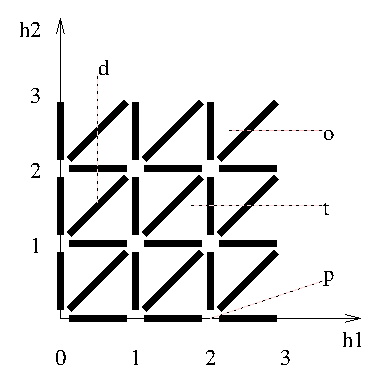
\includegraphics[width=.4\linewidth]{METHODS/regions.eps}
\end{center}
\caption{Clock regions on $\{h\protect_1, h\protect_2\}$ with $c\protect_1 = c\protect_2 = 2$\label{fig:regions}}
\end{figure}

 \subsection{Region Graph}\label{ss:mscregiongraph}
The region equivalence ${}\req{}$ over clock valuations can be
extended to an equivalence relation over the state space of $\AA$. Let
$(\States,\Init,\Labels,\TRel)$ be the transition system of $\AA$. Two
states from $\States$ are equivalent if they have identical locations
and their clock valuations are region equivalent. Formally, for
$(\tgloc,\clkvl), (\tgloc',\clkvl') \in \States$, $(\tgloc,\clkvl)
\req (\tgloc',\clkvl')$ iff $\tgloc = \tgloc'$ and $\clkvl \req
\clkvl'$. The region (equivalence class) of $\state =
(\tgloc,\clkvl)$ is denoted $\region{\state}$. The key property of
region equivalence is its \emph{stability} with respect to the 
transition relation of $\AA$, stated as follows:
\begin{proposition}[Stability of region equivalence]
Let $\TSys{\AA} = (\States,\Init,\Actions \cup \Time, \TRel)$ be the
transition system of $\AA$. Let $\state_1 \req \state_2$.
\begin{enumerate}
\item For all $a \in \Actions$, whenever $\state_1 \goes{a} \state'_1$,
there exists $\state'_2$ such that $\state_2 \goes{a} \state'_2$ and
$\state'_1 \req \state'_2$.
\item For all $t \in \Time$, whenever $\state_1 \goes{t} \state'_1$,
there exists $\state'_2$ and $t' \in \Time$ such that 
$\state_2 \goes{t'} \state'_2$, and $\state'_1 \req \state'_2$.
\qed
\end{enumerate}
\end{proposition}
We can gain an informal understanding of stability by considering
again the regions of Figure~\ref{fig:regions}. A state change can
occur either through a discrete transition or a time transition. For a
discrete transition, if two states are in the same region then they
satisfy the same set of guards and so if the transition is possible
for one state then it is also possible for the other. In taking the
transition, one or more of the clocks $\clock_1, \clock_2$ may be set
to $0$. Assume that $\clock_2$ is reset. This give a projection onto
the $\clock_1$ axis.  It can be seen that equivalent states are
projected to equivalent states.  For a time transition, since both $\clock_1$
and $\clock_2$ increase at the same rate, the state change occurs along the
diagonal at $45^\circ$ to the $\clock_1$ axis. Again it can be seen that for
any region and any pair of states within it, the sequence of regions 
encountered on the diagonal is the same.

\begin{definition}[Region Graph~{\rm\cite{acd:93,yov:97}}]
Let $\TSys{\AA} = (\States,\Init,\Actions \cup \Time,\TRel)$. Let
${}\req{}$ be a region equivalence for $\AA$ over $\States$. Let
$\tau \notin \Actions$ and $\Actions_\tau = \Actions \cup \{\tau\}$.
The \emph{region graph} $\RG(\AA)$ is given by 
$(\States_\req, \region{\Init}, \Actions_\tau, \goesRG{})$ where
\begin{enumerate}
\item $\States_\req = \{ \region{\state} | \state \in \States\}$
\item $\goesRG{} \subseteq \States_\req \cross \Actions_\tau \cross 
\States_\req$ is such that
\begin{enumerate}
\item for all $a \in \Actions$ and for all $\reg, \reg' \in \States_\req$,
$\reg \goesRG{a} \reg'$ iff there exists $\state, \state' \in \States$ such that
$\reg = \region{\state}$, $\reg' = \region{\state'}$, and $\state \goes{a} \state'$.
\item for all $\reg, \reg' \in \States_\req$, $\reg \goesRG{\tau} \reg'$ iff
\begin{enumerate}
\item $\reg = \reg'$ is an unbounded region, or
\item $\reg \neq \reg'$ and there exists $\state, \state' \in \States$ and 
$t \in \Time$ such that $\state \goes{t} \state'$, and $\reg = \region{\state}$
and $\reg' = \region{\state'}$, and for all $t' \in \Time$, if $t' \leq t$
then $\region{\state + t}$ is either $\reg$ or $\reg'$. 
\qed
\end{enumerate}
\end{enumerate}
\end{enumerate} 
\end{definition}
In the region graph, the passage of time is indicated by the occurrence of
a $\tau$-transition which records the fact that time has passed but abstracts
the exact amount of time elapsed. $\RG(\AA)$ is known as
a \emph{time-abstract} transition system. 

From the stability of the region equivalence, it is clear that a state
$\state'$ is reachable from a state $\state$ in the transition system
of $\AA$ iff $\region{\state'}$ is reachable from $\region{\state}$ in
the region graph of $\AA$. It is also clear that $\RG(\AA)$ is finite
since $\States_\req = \{(\tgloc,\region{\clkvl}) | \tgloc \in \tglocs
\land \clkvl \in
\clkvls \land \clkvl \models
\tginv(\tgloc)\}$ is finite, $\Actions_\tau$ is finite and therefore 
$\goesRG{} \subseteq \States_\req \cross \Actions_\tau \cross \States_\req$
is finite. It follows that reachability can be decided automatically by
constructing and searching the region graph. Both forward and backward
traversals of the region graph lead to effective algorithms. For example,
a method based on forward traversal consists in starting from
$\region{\state}$ and visiting the set of its successors and the 
successors of those and so on, until all reachable regions have been
visited. In this way, we construct the sequence 
$\Z_0 \subseteq \Z_1 \subseteq \cdots$, such that
\begin{eqnarray*}
\Z_0 & = & \region{\state} \\
\Z_{i+1} & = & Z_i \cup \{\reg | \exists \reg_i \in \Z_i \such \reg_i \goesRG{} \reg \}
\end{eqnarray*} 
Assume that $\Z = \lim_{i \geq 0} \Z_i$. Then, 
$\region{\state'}$ is reachable from $\region{\state}$ iff 
$\region{\state'} \in \Z$.
 
\subsection{Complexity of reachability}
A timed automaton $\AA$ with $m$ locations and $n$ clocks, in which
$c \geq \cmax(\AA)$, gives rise to a region graph with at most $m \cdot
n! \cdot 2^n \cdot (2c + 2)^n$ nodes. This bound is linear in the
number of locations but exponential both in the number of clocks and
the size of the constants appearing in the clock constraints. It can
be shown that the number of edges in the region graph is similarly
related to the number of locations and clocks and the size of
constants~\cite{ad:94}. In order to determine if a state $\state$ is
reachable in $\TSys{\AA}$, we search the region graph to see if
$\region{\state}$ is reachable in $\RG(\AA)$ --
Figure~\ref{fig:rgreach} outlines an algorithm to achieve this. Such a
search is linear in the number of nodes and edges of the region
graph. Therefore, the complexity of the reachability problem for $\AA$
is linear in the number of locations, exponential in the number of
clocks and exponential in the size of the constants in the clock
constraints. Formally, the problem is shown to be
PSPACE-complete~\cite{ad:94}. In fact, it is usually the case, in
practice, that $\AA$ is a product of component automata, so the region
graph can be seen as being exponential also in the number of component
automata. To summarise the causes of complexity, we can identify the
following factors:
\begin{enumerate}
\item the number of component automata
\item the number of clocks
\item the size of the constants in the clock constraints
\end{enumerate}
\begin{figure}
\begin{center}
\small
\begin{programbox}
|VISITED| := \{(\tgiloc, \region{\iclkvl})\}
|WAITING| := \{(\tgiloc, \region{\iclkvl})\}
\WHILE |WAITING| \neq \emptyset \DO
    \text{remove some } \reg \text{ from }  |WAITING|
    |succ| := \{\reg_s \vbar \reg \goesRG{} \reg_s\}
    \FOREACH \reg_s \in |succ| \DO
      \IF \reg_s \notin |VISITED|  
        \text{add } \reg_s\ \text{ to } |VISITED|
        \text{add } \reg_s\ \text{ to } |WAITING|
      \FI  
    \OD
\OD
\end{programbox}
\end{center}
\caption{Region graph reachability\label{fig:rgreach}}
\end{figure}
The combination of these factors cause a rapid growth in the number of
states which must be considered, as the size of the problem
description increases. This rapid growth is known as the \emph{state
explosion problem} and is currently the most challenging of the
technical difficulties to be addressed in the application of automated
analysis to formal verification problems in the analysis of real-time systems. 
\subsubsection{The state explosion problem}
Consider again the algorithm for generating reachable regions in
Figure~\ref{fig:rgreach}. It can be seen that the algorithm stores each
region from the region graph in the set $VISITED$. For the purposes of this
algorithm, a `state' is equated with a region. Storing the set of
$VISITED$ states makes termination of the algorithm easy to
determine and ensures that states are not explored (have their
successors generated) more than once. However, because the number of
states can be very large, the available computational resources may
become exhausted before the problem is solved. A number of attacks on
the state explosion problem can be suggested:
\begin{enumerate}
\item generate fewer `states',
\item store fewer `states',
\item compress the `state' store so that it requires less memory.
\end{enumerate}
Such methods may be orthogonal and so can be combined to produce even
greater benefits.  In the following section, we consider one such
approach which has proven successful in practice and is the basis for
some of the most effective verification tools currently in use.

\subsection{Constraint Solving}\label{ss:mscconstraint}
The partitioning of the space of clock valuations which arises in the
construction of the region graph, although finite, is very
fine-grained.  Consequently, implementations based directly on the
region graph turn out to be not very efficient. In~\cite{hnsy:94} a
symbolic technique was proposed which works directly with the clock
constraints which arise in the calculation of discrete- and
time-predecessors (and successors). This technique leads to a much
coarser partitioning of the state space. The method of~\cite{hnsy:94}
works in a `backward' manner, whereby starting from a set of target
locations, the set of all states from which it is possible to reach
those locations is calculated -- it is then simple to test if an
initial state lies within this set. In fact, this method is used in
solving the model-checking problem for TCTL rather than simple
reachability. The main problems with a backward traversal of the state space
are:
\begin{itemize}
\item the whole of the potential state space may be considered rather than
just that part which is reachable from an initial state;
\item an answer cannot be returned until the complete state space 
exploration terminates;
\item it is not easy to provide a diagnostic trace in the case that a 
violating state is found to be reachable.
\end{itemize}
The idea of working symbolically with clock constraints
in a `forward' manner seems to have arisen independently, at about the
same time, in several groups~\cite{acd:92,oli:94,ypd:94}. This approach
is often more efficient in practice, allows for a diagnostic trace to be
provided when a property is found to be violated and is the basis of 
successful implementations~\cite{bll:95,dot:95}. We rely on `forward'
constraint solving techniques in Chapter~\ref{chap:sggen} and provide an
introduction below.  

\subsubsection{Symbolic states}
A node in the region graph of a TA $\AA$ is a `symbolic' state which
represents a (possibly infinite) number of states in the transition
system of $\AA$. Each node is of the form $(\tgloc, \reg)$ where
$\tgloc$ is a location of $\AA$ and $\reg$ is a clock region. Such a
symbolic state represents the set of states $(\tgloc,\clkvl)$ where
$\clkvl \in \reg$. We have seen that every clock region can be
characterised by a clock constraint, so a node $(\tgloc,\reg)$ can be
written as $(\tgloc,\clkcond)$ where $\clkcond$ is the characteristic
formula of the region $\reg$. This idea can be extended by allowing
$\clkcond$ to be a constraint which characterises a \emph{union} of
perhaps many clock regions. Formally, a symbolic state is defined
as follows.
\begin{definition}[Symbolic state]
Let $\AA = (\tglocs,\tgiloc,\Actions,\tgclks,\tgedges,\tginv)$ be a 
timed automaton. A \emph{symbolic state} of $\AA$ is a pair 
$(\tgloc,\clkcond)$ where $\tgloc \in \tglocs$ is a location of $\AA$
and $\clkcond \in \ClockConstraints$ is a clock constraint.

The meaning of a  symbolic state $(\tgloc,\clkcond)$, denoted 
$\chset{(\tgloc,\clkcond)}$, is the set of states
$\{(\tgloc,\clkvl) | \clkvl \models \clkcond\}$.  
\qed
\end{definition}

Let $\Z$ be a set of symbolic states. We denote by $\chset{\Z}$ the
set $\bigcup \{\chset{(\tgloc,\clkcond)} | (\tgloc,\clkcond) \in
\Z\}$ and by $\locations(\Z)$ the set of locations 
$\{\tgloc | \exists \clkcond \in \ClockConstraints \such (\tgloc,\clkcond) \in \Z\}$. 

The state space may be covered by a much smaller set of symbolic
states of this form, and so the problem of state space explosion may be
mitigated to some extent.  In particular, a set of regions $\Z$ can be
represented as a \emph{united} set of symbolic states $\Z' =
\{(\tgloc,\clkcond_\tgloc) | \tgloc \in \tglocs \land \clkcond_\tgloc
\in \ClockConstraints\}$ in which there is at most one element 
$(\tgloc,\clkcond_\tgloc)$ for each location $\tgloc$, and
$\clkcond_\tgloc$ is the characteristic formula for the set of \emph{all}
clock regions in $\Z$ which are paired with the location~$\tgloc$. 

Let $\Z$ be a set of symbolic states. We denote by
$\clkcond_\tgloc^\Z$ the clock constraint characterising the set of 
clock valuations associated with $\tgloc$ in $\Z$, i.e.,
$\chset{\clkcond_\tgloc^\Z} = \bigcup\{\chset{\clkcond} | (\tgloc,\clkcond) \in \Z \}$.
We use $\unite(\Z)$ to denote the set 
$\{(\tgloc, \clkcond_\tgloc^\Z) | \tgloc \in \locations(\Z)\}$, and
$\Z_1 \uplus \Z_2$ to denote
$\unite (\Z_1 \cup \Z_2)$ and $\biguplus_{i \in I} \Z_i$ to denote
$\unite(\bigcup_{i \in \I} \Z_i)$.

In the following section, we discuss the calculation of the discrete
and time-successors of symbolic states, and show how united sets of
symbolic states can be used in the forward computation of reachable
states.

\subsubsection{Forward computation of clock constraints}
Let $\tgloc \in \tglocs$, $\clkcond \in \ClockConstraints$ and
$\tgedge = (\tgloc,\tgguard,a,\someclks,\tgloc') \in \tgedges$.
We consider predicate transformers $\suc{\tgedge}{}(\clkcond)$ and
$\suc{\tau}{\tgloc}(\clkcond)$ which are needed in the calculation of discrete
and time-successors, respectively, of a symbolic state
$(\tgloc,\clkcond)$. 

On the one hand, $\suc{\tgedge}{}(\clkcond)$ denotes a clock constraint
over $\tgclks$ which characterises the set of clock valuations which
are reachable from the clock valuations in $\clkcond$ when a discrete
transition is taken via the edge $\tgedge$, i.e.,
$\suc{\tgedge}{}(\clkcond)$ denotes a predicate satisfying
\begin{zed}
 \chset{\suc{\tgedge}{}(\clkcond)} =
  \{\clkvl[\someclks:=0] | \clkvl \in \clkvls 
  \land (\clkvl \models \clkcond \land \tgguard)
  \land \clkvl[\someclks:=0] \models \tginv(\tgloc')\} 
\end{zed}

On the other hand, $\suc{\tau}{\tgloc}(\clkcond)$ denotes a clock constraint
over $\tgclks$ which characterises the set of clock valuations which are
reachable from the clock valuations in $\clkcond$ as time passes while
control resides at $\tgloc$, i.e., $\suc{\tau}{\tgloc}(\clkcond)$ denotes
a predicate satisfying
\begin{zed}
  \chset{\suc{\tau}{\tgloc}(\clkcond)} =
  \{\clkvl + t | \clkvl \in \clkvls \land t \in \Time \land \clkvl \models \clkcond \land \\
\t3 \forall t' \in \Time \such t' \leq t
    \implies \clkvl + t' \models \tginv(\tgloc)\}  
\end{zed}   

Together, $\suc{\tgedge}{}(\clkcond)$ and $\suc{\tau}{\tgloc}(\clkcond)$
can be used in solving the reachability problem by computing
the sequence of sets of symbolic states $\Z_0, \Z_1, \cdots$ as
follows:
\begin{eqnarray*}
\Z_0 & = & \{(\tgloc,\clkcond)\} \\ 
\Z_{i+1} & = & \{(\tgloc',\suc{\tgedge}{}(\clkcond)) |
                  (\tgloc,\clkcond) \in \Z_i \land 
                  \tgedge = (\tgloc,\tgguard,a,\someclks,\tgloc') \in 
                  \tgedges\} \uplus \\
         &   & \{(\tgloc,\suc{\tau}{\tgloc}(\clkcond)) | (\tgloc,\clkcond) \in
                  \Z_i\}  
\end{eqnarray*} 

Notice that $\Z_i \subseteq \{(\tgloc,\suc{\tau}{\tgloc}(\clkcond)) |
(\tgloc,\clkcond) \in \Z_i\}$. Let $\Z = \lim_{i \geq 0} \Z_i$. All
states in a symbolic state $(\tgloc',\clkcond')$ are reachable from
some state in $(\tgloc,\clkcond)$ iff $(\tgloc',\clkcond'') \in \Z$
and $\chset{\clkcond'} \subseteq \chset{\clkcond''}$, i.e.,
$\clkcond'$ implies $\clkcond''$.
  
\subsubsection{Implementing the constraint solving approach}
In order to exploit these ideas in practice, it is necessary to see
how it is possible to represent clock constraints and to implement the
operations $\uplus$, $\suc{\tgedge}{}$ and $\suc{\tau}{}$ using this
representation. As a first step, we observe that $\ClockConstraints$
is closed under these operations for any timed automaton, i.e., the
operations are always well-defined -- the reader is referred
to~\cite{oli:94} for a proof. Next, we note that the adoption of a
`geometric' perspective leads to natural definitions of many of the
operations which are needed and helps in acquiring an intuitive
understanding of them. We follow this approach below.

\subsubsection{Polyhedra}
Let $\clocks = \{\clock_1,\clock_2,\ldots,\clock_n\}$ be a set of
clocks.  A union of $\clocks$-regions is a \emph{$\clocks$-polyhedron}
in the $n$-dimensional Euclidean space, where a $\clocks$-polyhedron
is simply the set of $\clocks$-valuations satisfying a clock
constraint $\clkcond \in \ClockConstraints$. It is often convenient,
notationally, to identify a constraint with 
the $\clocks$-polyhedron which it defines, and so,
for example, we will write $\clkvl \in \clkcond$ for 
$\clkvl \in \chset{\clkcond}$, or $\clkcond_1 \cup \clkcond_2$ for
$\chset{\clkcond_1} \cup \chset{\clkcond_2}$.

A polyhedron is said to be \emph{convex}, if for any two points within
it, all points on the line segment joining them are also within it.
Formally, a $\clocks$-polyhedron $\vexcond$ is
convex iff for any $\clkvl_1,
\clkvl_2 \in \vexcond$ and $t \in \Time$ such that $0 < t < 1$, we have
$t\cdot\clkvl_1 + (1 - t) \cdot \clkvl_2 \in \vexcond$. This means that
if $\clkvl$ and $\clkvl + t$ are clock valuations, both of which lie
within a convex polyhedron $\clkcond$, then all valuations $\clkvl + t'$,
where $t' \leq t$, also lie within $\clkcond$.   

It can be shown that the set of convex $\clocks$-polyhedra coincides
with the set $\ClockZones$ of clock zones, i.e., any convex
$\clocks$-polyhedron can be expressed as a conjunction of atomic
constraints, and any conjunction of atomic constraints defines a
convex $\clocks$-polyhedron. Note that any non-convex
$\clocks$-polyhedron, $\clkcond$, can be expressed as the union of a
finite set of convex $\clocks$-polyhedra,
$\bigcup\{\vexcond_1,\vexcond_2,\ldots,\vexcond_m\}$.
\begin{exampleb}
Figure~\ref{fig:polyexs} shows (a) one convex and (b,c) two non-convex
polyhedra, which are unions of clock regions and are defined by the
constraints:
\begin{enumerate}
\item[a)] $1 \leq h_1 \leq 3 \land 1 \leq h_2 \leq 3 \land -1 \leq h_2 - h_1\leq 1$
\item[b)] $(0 \leq h_1 \leq 3 \land 0 \leq h_2 \leq 1 \land 0 \leq h_1 - h_2 \leq 2) \lor$ \\ $(1 \leq h_1 \leq 2 \land 2 \leq h_2 \leq 3)$
\item[c)] $(0 \leq h_1 \leq 1 \land 1 \leq h_2 \leq 3) \lor$ $(1 \leq h_1 \leq 2 \land 1 \leq h_2 \leq 2)$
\qed
\end{enumerate}
\end{exampleb}
\begin{figure}
\begin{center}
\psfrag{h1}{$h_1$}
\psfrag{h2}{$h_2$}
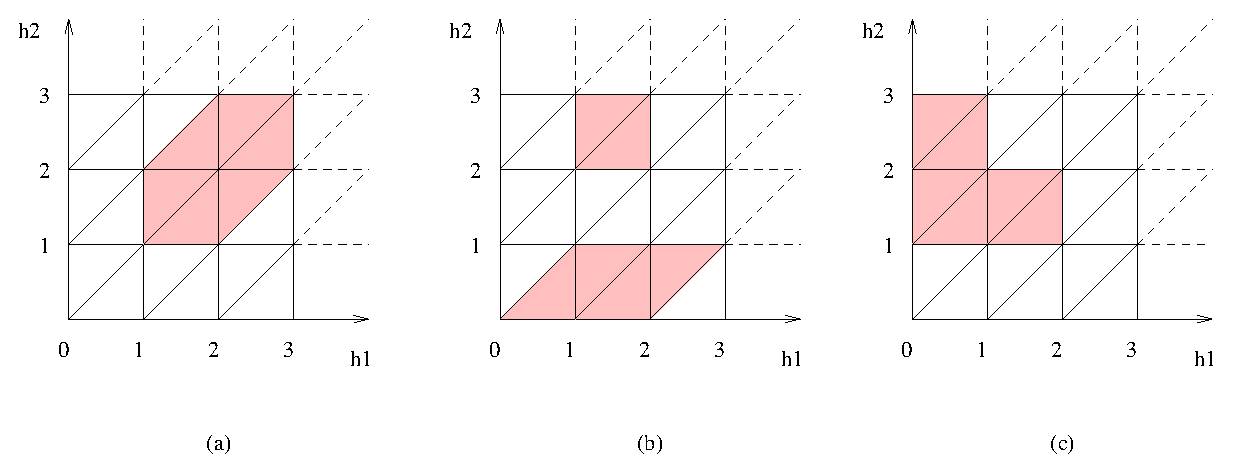
\includegraphics[width=\linewidth]{METHODS/polyexs.eps}
\end{center}
\caption{Convex and Non-convex Polyhedra\label{fig:polyexs}}
\end{figure}

\subsubsection{Operations on polyhedra} \label{ss:polyops}
In this section, we define a number of operations on polyhedra which
are needed in the rest of the dissertation. Some of the operations are
illustrated in Figure~\ref{fig:polyops} where the result of
each operation is indicated by the shaded part in each case. 

\begin{paragraph}{Basic operations}
\emph{Intersection}, \emph{union} and \emph{complementation} are given
immediately by conjunction, disjunction and negation respectively, i.e.,
$\clkcond_1 \cap \clkcond_2 = \{\clkvl \in \clkvls | \clkvl
\models \clkcond_1 \land \clkcond_2\}$,
$\clkcond_1 \cup \clkcond_2 = \{\clkvl \in \clkvls | \clkvl \models
\clkcond_1 \lor \clkcond_2\}$ and $\overline{\clkcond} = \{\clkvl \in \clkvls
| \clkvl \models \lnot \clkcond\}$ -- examples of intersection and union
are given in Figures~\ref{fig:polyops}(a) and (b), respectively.
\emph{Difference} is defined
as usual by $\clkcond_1 \setminus \clkcond_2 = \clkcond_1 \cap
\overline{\clkcond_2}$ and the \emph{inclusion}  
$\clkcond_1 \subseteq \clkcond_2$ is equivalent to $\clkcond_1
\setminus \clkcond_2 = \emptyset$. 
\end{paragraph}

\begin{paragraph}{Convex hull}
The \emph{convex hull} of two $\clocks$-polyhedra $\clkcond_1$
and $\clkcond_2$ is denoted $\clkcond_1 \hull \clkcond_2$, and is 
defined to be the smallest convex $\clocks$-polyhedron $\vexcond$ which
contains both $\clkcond_1$ and $\clkcond_2$, i.e.,
$\clkcond_1 \subseteq \vexcond$ and $\clkcond_2 \subseteq \vexcond$.
Figure~\ref{fig:polyops}(c) gives an example of the convex hull operation. 
\end{paragraph}

\begin{figure}
\begin{center}
\psfrag{h1}{$h_1$}
\psfrag{h2}{$h_2$}
\psfrag{Z}{$\clkcond$}
\psfrag{Z1}{$\clkcond_1$}
\psfrag{Z2}{$\clkcond_2$}
\psfrag{Z1iiZ2}{$\clkcond_1 \cap \clkcond_2$}
\psfrag{Z1uZ2}{$\clkcond_1 \cup \clkcond_2$}
\psfrag{Z1hZ2}{$\clkcond_1 \hull \clkcond_2$}
\psfrag{Zfp}{$\forwardproj{\clkcond}$}
\psfrag{Zrst}{$\clkcond[h_2:=0]$}
\psfrag{Zcls}{$\close{c}{\clkcond}$}
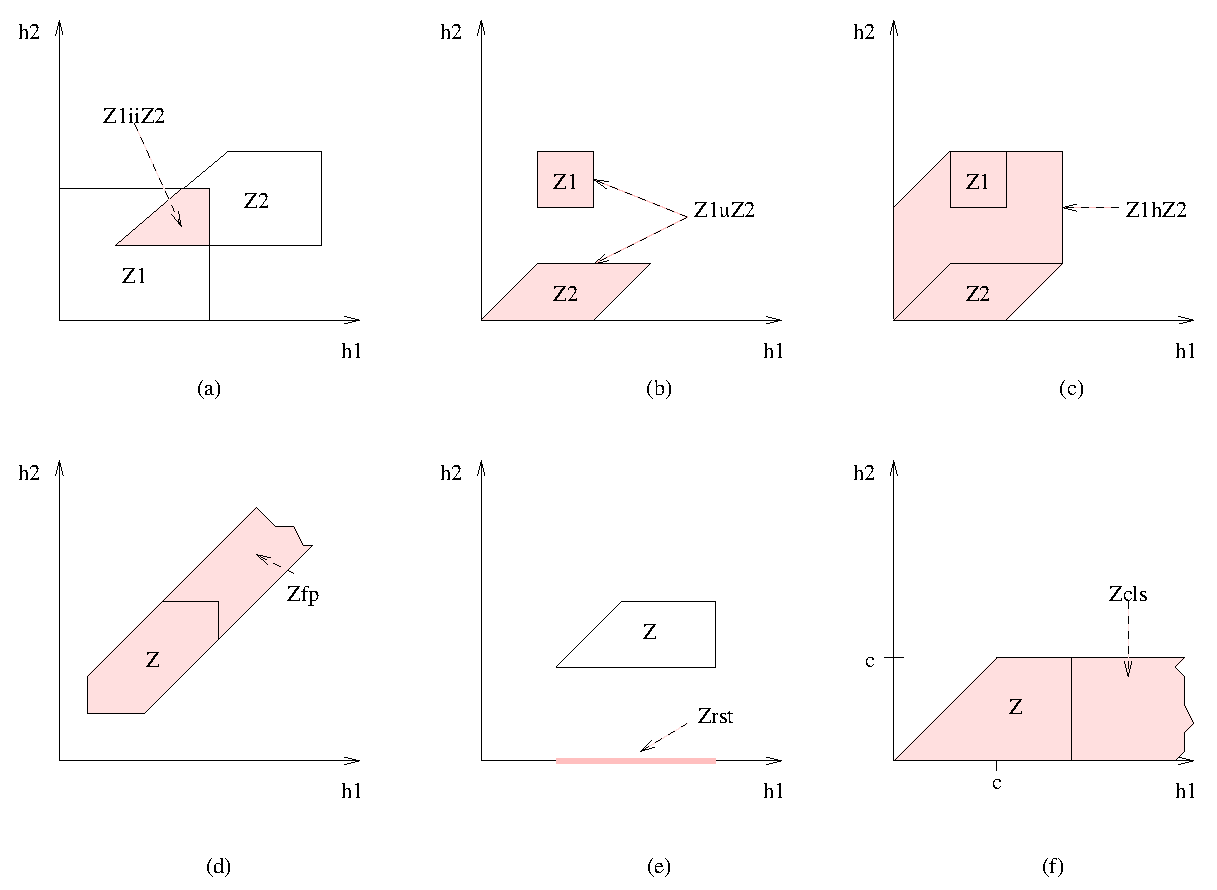
\includegraphics[width=\linewidth]{METHODS/polyops.eps}
\end{center}
\caption{Operations on Polyhedra\label{fig:polyops}}
\end{figure}

\begin{paragraph}{Projections} The \emph{forward projection} of a 
$\clocks$-polyhedron $\clkcond$, denoted $\forwardproj{\clkcond}$, is
the largest set of $\clocks$-valuations which can be obtained from the
valuations in $\clkcond$ by the passage of time. Formally,
\[ \forwardproj{\clkcond} \defs \{\clkvl + t | \clkvl \in \clkcond \land 
   t \in \Time\} \] 
For a polyhedron $\clkcond$ on
$\{\clock_1,\clock_2\}$, since $\clock_1$ and $\clock_2$ advance
together in lock-step with the passage of time, the forward projection
$\forwardproj{\clkcond}$ encompasses all those valuations which can be
reached from a valuation in $\clkcond$ by following the diagonal at
$45^\circ$ to the horizontal axis. Figure~\ref{fig:polyops}(d) shows
an example.

The operation giving the \emph{reset successors} of a
$\clocks$-polyhedron $\clkcond$, for a given reset set $\someclks
\subseteq \clocks$, is denoted $\clkcond[\someclks := 0]$ and is
defined by:
\[ \clkcond[\someclks := 0] \defs \{\clkvl[\someclks := 0] | \clkvl \in \clkcond\} \]
Intuitively, the reset of a clock $\clock_2$, for a polyhedron
$\clkcond$, involves a projection of $\clkcond$ onto the $\clock_1$ axis -- see
Figure~\ref{fig:polyops}(e).
\end{paragraph}

\begin{paragraph}{$c$-closure}
The operation of $c$-closure, defined on convex polyhedra, is based on
the idea that if the value of some clock exceeds a specified constant
$c$ in each of two clock valuations, then that clock is not regarded
as significant in distinguishing between them. The $c$-closure
operation is used to ensure the finiteness of partitionings of the
infinite space of clock valuations. We have seen a similar idea
already in connection with the region
graph~(\Sec\ref{ss:mscregiongraph}). $c$-closure appears in the literature
under a variety of names, e.g., \emph{rounding}~\cite{wt:95},
\emph{extrapolation}~\cite{dt:98} and \emph{normalisation}~\cite{pet:99}. 
The definition given here follows~\cite{tri:98}.

Let $c \in \nat$ and $\clkvl,\clkvl' \in \clkvls$. We say that
$\clkvl$ and $\clkvl'$ are \emph{$c$-equivalent} if:
\begin{enumerate}
\item for any clock $\clock$, either $\clkvl(\clock) = \clkvl'(\clock)$,
  or $\clkvl(\clock) > c$ and $\clkvl'(\clock) > c$, and
\item for any pair of clocks, $\clock_1, \clock_2$, either
  $\clkvl(\clock_1) - \clkvl(\clock_2) = \clkvl'(\clock_1) - \clkvl'(\clock_2)$, or $\clkvl(\clock_1) - \clkvl(\clock_2) > c$ and $\clkvl'(\clock_1) - \clkvl'(\clock_2) > c$. 
\end{enumerate}
For a convex $\clocks$-polyhedron $\vexcond$, the
$c$-closure of $\vexcond$, denoted $\close{c}{\vexcond}$, is defined to be the
greatest convex $\clocks$-polyhedron $\vexcond' \supseteq \vexcond$,
such that for all $\clkvl' \in \vexcond'$ there exists $\clkvl \in \vexcond$
and $\clkvl$, $\clkvl'$ are $c$-equivalent. $\vexcond$ is said to be $c$-closed
if $\close{c}{\vexcond} = \vexcond$. Figure~\ref{fig:polyops}(f) shows an
example of $c$-closure.
\begin{proposition}\label{prop:cclosure}
$c$-closure satisfies the following properties:
\begin{enumerate}
\item If $\vexcond$ is $c$-closed then it is $c'$-closed, for any
  $c' \geq c$.
\item If $\vexcond_1$ and $\vexcond_2$ are $c$-closed then $\vexcond_1 \cap
  \vexcond_2$ is also $c$-closed.
\item For any $\vexcond$, there exists a constant $c$ such that 
  $\vexcond$ is $c$-closed.
\item For any constant $c$, there is a finite number of $c$-closed
  convex $\clocks$-polyhedra.
\end{enumerate}
\end{proposition}
\begin{proof}
cf. Tripakis~\cite{tri:98}
\end{proof}
\end{paragraph}

\subsubsection{Properties of polyhedral operations}
Firstly, we identify those operations of the previous section which
preserve convexity.
\begin{proposition}\label{prop:polyconvex}
Let $\vexcond, \vexcond_1, \vexcond_2$ be convex $\clocks$-polyhedra.
Let $\someclks \subseteq \clocks$ and $c \in \nat$. Then, $\vexcond_1
\cap \vexcond_2$, $\vexcond_1 \hull \vexcond_2$,
$\forwardproj{\vexcond}$, $\vexcond[\someclks:=0]$ and
$\close{c}{\vexcond}$ are all convex.
\end{proposition}
\begin{proof}
cf. Tripakis~\cite{tri:98}
\end{proof}

\begin{proposition}\label{prop:polysuc}
Let $\AA$ be a timed automaton with a set $\clocks$ of clocks and
a set $\tgedges$ of edges with $\tgedge = (\tgloc,\tgguard,a,\someclks,\tgloc') \in \tgedges$. Let $\clkcond$ be a $\clocks$-polyhedron.
The following equalities hold. 
\begin{eqnarray*}
  \suc{\tgedge}{}(\clkcond) & = & ((\clkcond \cap \tgguard)[\someclks:=0]) \cap \tginv(\tgloc') \\ 
  \suc{\tau}{\tgloc}(\clkcond) & = & \forwardproj{\clkcond} \cap \tginv(\tgloc)\end{eqnarray*}
\end{proposition}
\begin{proof}
The equalities can be derived directly from the definitions of
$\suc{\tau}{}$, $\suc{\tgedge}{}$ and the polyhedral operations.
\end{proof}

Proposition~\ref{prop:polysuc} leads some way towards an
implementation of the constraint-solving approach.  In order to make
further progress, we need to define an efficient representation for
clock constraints and show how the polyhedral operations can be
implemented on it. It is also necessary to consider the implications
of the use of the $\uplus$ operator, which, in the general case, gives
rise to non-convex polyhedra. The issues raised by this consideration
are more easily discussed following the introduction of the
\emph{difference bound matrix} representation of clock constraints
which is presented in the following section.

\subsection{Difference Bound Matrices} \label{ss:mscdbm}
The efficient implementation of algorithms for automatic analysis
based on constraint solving relies upon a representation of polyhedra
which is compact and which supports the operations identified in
section~\ref{ss:polyops}. Dill~\cite{dil:89} introduced
\emph{difference bound matrices} (DBMs) for this purpose\footnote{In
fact, the data structure was known many years earlier~\cite{bel:57}
and later had been used in the analysis of Time Petri
nets~\cite{mb:83} but Dill's paper revived interest and pointed the
way to their use in the analysis of timed automata.} and this data
structure remains pre-eminent in the implementation of analysis tools
for dense-time systems -- KRONOS and UPPAAL are examples. We now
present those details of DBMs and their use which will be needed later
in the dissertation; more detailed presentations, including
proofs, can be found in~\cite{dil:89,oli:94,tri:98,yov:93,yov:97}.

\subsubsection{Bounds}
A \emph{bound} is a pair $(c,\brel) \in \Zinf \cross \{<, \leq\}$,
where $\Zinf = \num \cup \{\infinity\}$. Bounds are ordered as follows:
$c < \infinity$, for any $c \in \num$, and  $<$ is strictly less than $\leq$;
we then take the usual lexicographic ordering where for all 
$(c,\brel),(c',\brel') \in \Zinf \cross \{<,\leq\}$, $(c,\brel) < (c',\brel')$
if either $c < c'$, or $c = c'$ and $\brel < \brel'$. 
$(c,\brel) \leq (c',\brel')$ if $(c,\brel) < (c',\brel')$ or $c = c'$ and 
$\brel = \brel'$.

The \emph{minimum} of two bounds $(c,\brel), (c',\brel')$, denoted
$\min((c,\brel),(c',\brel'))$, is $(c,\brel)$ if 
$(c,\brel) \leq (c',\brel')$ and $(c',\brel')$ otherwise. 
The \emph{maximum} of two bounds $(c,\brel), (c',\brel')$, denoted
$\max((c,\brel),(c',\brel'))$, is $(c,\brel)$ if 
$(c',\brel') \leq (c,\brel)$ and $(c',\brel')$ otherwise. 
The \emph{addition} of bounds is defined by the following table:
\begin{center}
\begin{tabular}{|>{$}c<{$}|>{$}c<{$}>{$}c<{$}|}
\hline
+ & (c',\leq) & (c',<) \\
\hline
(c,\leq) & (c+c',\leq) & (c+c',<) \\
(c,<) & (c+c',<) & (c+c',<) \\
\hline
\end{tabular}
\end{center}
Note that as usual $c + \infinity = \infinity + c = \infinity$ for any 
$c \in \Zinf$. 

\subsubsection{Representation of convex polyhedra}
Let $\clocks = \{\clock_1,\clock_2,\ldots,\clock_n\}$ be a set of
clocks.  The set $\ClockZones$ of convex $\clocks$-polyhedra contains
elements which are given as the conjunction of atomic constraints.  An
atomic constraint of the form $\clock_i - \clock_j \brel c$ can be
represented by associating the bound $(c, \brel)$ with the pair of
clocks $\clock_i, \clock_j$. A constraint such as $\clock_i - \clock_j
\geq c$ is equivalent to $\clock_j - \clock_i \leq -c$ and so can be 
represented by associating the bound $(-c,\leq)$ with
$\clock_j,\clock_i$.  In order to achieve a uniform representation, a
new fictitious clock variable $\clock_0$ is introduced to represent
the constant $0$. This allows constraints such as $\clock_i \brel c$
to be represented as $\clock_i - \clock_0 \brel c$.  In this way, a
convex $\clocks$-polyhedron can be encoded as a $(n + 1)
\times (n + 1)$ square matrix $\M$ whose elements are bounds. Such a matrix 
is said to have \emph{dimension} $n$. The element $\M_{i,j}$ gives the
upper bound on the clock difference $\clock_i - \clock_j$. For
example, the constraint $\clock_2 < 9$ is encoded as $\M_{2,0} =
(9,<)$ and $\clock_5 \geq 6$ by $\M_{0,5} = (-6,\leq)$. If $\clock_i
-\clock_j$ is unbounded then we set $\M_{i,j} = (\infinity, <)$. The
set of $\clocks$-valuations defined by the DBM $\M$, denoted
$\chset{\M}$, is the set $\{\clkvl \in \clkvls | \forall i,j \in
\{0..n\} \such \M_{i,j} = (c,\brel) \implies \clkvl(\clock_i) -
\clkvl(\clock_j) \brel c\}$.  Notice that we silently extend $\clkvl$
by requiring $\clkvl(\clock_0) = 0$.

\begin{figure}
\begin{tabular}{ll}
\begin{tabular}{c}
\psfrag{h1}{$h_1$}
\psfrag{h2}{$h_2$}
\psfrag{a}{}
\psfrag{b}{}
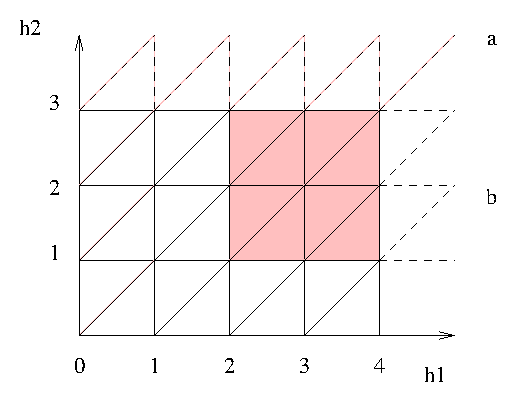
\includegraphics[width=.4\linewidth]{METHODS/dbm.eps}
\end{tabular}
&
\begin{tabular}{c}
\fbox{
\begin{math}
\begin{array}{cccc}
\M & \clock_0 & \clock_1 & \clock_2 \\
\clock_0 & (0,\leq) & (-2,\leq) & (-1,\leq) \\
\clock_1 & (4,\leq) & (0,\leq) & (\infinity,<) \\
\clock_2 & (3,\leq) & (\infinity,<) & (0,\leq)
\end{array}
\end{math}
} \\ \\
\fbox{
\begin{math}
\begin{array}{cccc}
\M' & \clock_0 & \clock_1 & \clock_2 \\
\clock_0 & (0,\leq) & (-2,\leq) & (-1,\leq) \\
\clock_1 & (4,\leq) & (0,\leq) & (3,\leq) \\
\clock_2 & (3,\leq) & (1,\leq) & (0,\leq)
\end{array}
\end{math}
} 
\end{tabular}
\end{tabular}
\caption{Representation of a convex polyhedron by DBM's\label{fig:dbm}}
\end{figure}

\begin{exampleb}
Let $\vexcond = 2 \leq \clock_1 \leq 4 \land 1 \leq \clock_2 \leq 3$
be a clock constraint.  Figure~\ref{fig:dbm} illustrates the convex
polyhedron defined by $\vexcond$ and the DBM $\M$ which represents it.
\qed
\end{exampleb}

\begin{figure}
\begin{center}
\psfrag{h0}{$h_0$}
\psfrag{h1}{$h_1$}
\psfrag{h2}{$h_2$}
\psfrag{c0}{$(0,\leq)$}
\psfrag{c1}{$(0,\leq)$}
\psfrag{c2}{$(0,\leq)$}
\psfrag{c01}{$(-2,\leq)$}
\psfrag{c10}{$(4,\leq)$}
\psfrag{c02}{$(-1,\leq)$}
\psfrag{c20}{$(3,\leq)$}
\psfrag{c12}{$(\infinity,<)$}
\psfrag{c21}{$(\infinity,<)$}
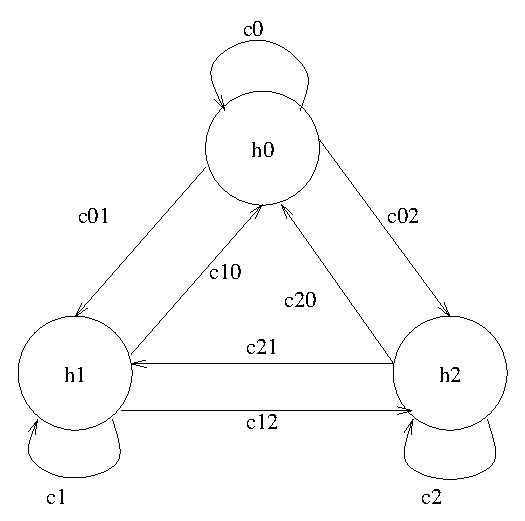
\includegraphics[width=.45\linewidth]{METHODS/dbmgraph.eps}
\end{center}
\caption{Weighted graph interpretation of a DBM\label{fig:dbmgraph}}
\end{figure}

A DBM can also be regarded as the adjacency matrix of a fully
connected, weighted directed graph, where each clock is a node in the
graph and each entry $\M_{i,j}$ gives the weight on the arc from
$\clock_i$ to $\clock_j$. Figure~\ref{fig:dbmgraph} shows the weighted
graph corresponding to DBM $\M$ in Figure~\ref{fig:dbm}.  We will use
this interpretation whenever it is convenient in a given context.

Notice that there may be many DBMs which represent a given convex
polyhedron, i.e., the representation is not unique. This can be
observed in Figure~\ref{fig:dbm} where $\M'$ represents the same
polyhedron as $\M$. A canonical representation is desirable since it
allows certain semantic operations on polyhedra -- the testing of
equality, emptiness and inclusion, for example -- to be reduced to syntactic
operations on DBMs. An ordering on DBMs is induced by the ordering on
bounds: $\M \leq \M'$ iff $\M_{i,j} \leq M'_{i,j}$, for all $0 \leq
i,j \leq n$ where $n$ is the dimension of $\M$ and $\M'$. This
ordering allows a \emph{canonical form} $\M_\vexcond$ to be defined
for any non-empty convex polyhedron $\vexcond$: we require that
$\M_\vexcond \leq \M$, for any DBM $\M$ representing $\vexcond$,
i.e., in the canonical form, all bounds are as `tight' as possible.  The
empty polyhedron is defined by any inconsistent set of constraints. We
choose its canonical form arbitrarily to be one of the many possible
representations, denoting it $\M^\emptyset$, where $\M^\emptyset_{i,j}
\defs (0,<)$, for $0 \leq i,j \leq n$. If $\M$ is a DBM, then $\canon(\M)$ 
denotes the canonical form of $\M$ and $\chset{\canon(\M)} = \chset{\M}$.
In Figure~\ref{fig:dbm}, $\M' = \canon(\M)$.
It is now simple to test if two matrices represent the same constraint:
$\M$ and $\M'$ represent the same constraint if $\canon(\M) = \canon(\M')$.

Notice that $\chset{\M^\emptyset} = \emptyset$ and so represents the
constraint $\ccfalse$. 
The \emph{universal} matrix $\UU$, which
imposes the minimal constraints that clock differences should be at least
$0$ and less than $\infinity$, is defined by: $\UU_{i,j} = (0,\leq)$ if
$i = 0$ or $i = j$ otherwise $\UU_{i,j} = (\infinity,<)$. $\chset{\UU}
= \clkvls$ and so represents the constraint $\cctrue$.

\subsubsection{Implementation of polyhedra operations} 
\begin{paragraph}{Canonical Form}
The canonical form $\M'$, of a DBM $\M$ of dimension $n$, can be
computed from the interpretation of $\M$ as a weighted directed graph
by requiring that, for all $0 \leq i,j \leq n$, the weight $\M'_{i,j} =
\min\{\weight_\M(\path) | \path \text{ is a path from } \clock_i
\text{ to } \clock_j\}$, where a path $\path$ from $\clock_i$ to 
$\clock_j$ is any sequence of nodes $\clock_i = \clock_{i_1},
\clock_{i_2},\ldots,\clock_{i_m} = \clock_j$ and its weight in $\M$, 
denoted $\weight_\M(\path)$, is given by $\M_{i_1,i_2} + \M_{i_2,i_3}
+ \cdots + \M_{i_{m-1},i_m}$.  If there is a cycle $\clock_i =
\clock_{i_1}, \clock_{i_2},\ldots,\clock_{i_m} = \clock_i$, such that 
$\weight_\M(\clock_{i_1},\clock_{i_2},\ldots,\clock_{i_m}) <
(0,\leq)$, then $\M$ represents the empty polyhedron --- clearly, it
cannot be the case that $\clock_i - \clock_i < 0$ --- and its canonical
form is $\M^\emptyset$, otherwise the canonical form of $\M$ is given
by $\M'$. We can calculate the canonical form of a DBM by using a
version of the Floyd-Warshall all-pairs shortest path algorithm, as
shown in Figure~\ref{fig:fw}.  It is apparent that the complexity of
the algorithm is $\bigO((n+1)^3)$ for a DBM of dimension $n$.
\begin{figure}
\begin{center}
\small
\begin{programbox}
\mkcanon(\M)
\BEGIN
\FOR k = 0 \TO n \DO
  \FOR i = 0 \TO n \DO
    \FOR j = 0 \TO n \DO
      \M_{i,j} := \min(\M_{i,j},\M_{i,k} + \M_{k,j})
    \OD
    \IF \M_{i,i} < (0,\leq) \THEN \RETURN \M^\emptyset \FI
  \OD
\OD
\RETURN \M   
\END
\end{programbox}
\end{center}
\caption{Procedure to compute the canonical form of a DBM\label{fig:fw}}
\end{figure}

\end{paragraph}
 
\begin{paragraph}{Intersection}
Given two DBMs $\M$ and $\M'$ of dimension $n$, representing the
convex polyhedra $\vexcond, \vexcond'$, respectively, then the intersection
$\vexcond \cap \vexcond'$ is represented by the DBM $\M''$,
where $\M''_{i,j} = \min(M_{i,j},\M'_{i,j})$ for $0 \leq i,j \leq n$.
This is true even if $\M$ and $\M'$ are not in canonical form. However,
$\M''$ is not necessarily in canonical form even if both $\M$ and $\M'$ are.
\end{paragraph}

\begin{paragraph}{Inclusion}
Let $\M$ and $\M'$ be the DBMs of dimension $n$ which are the
canonical representatives of the convex polyhedra $\vexcond$ and
$\vexcond'$, respectively. $\vexcond \subseteq \vexcond'$ iff $\M_{i,j}
\leq \M'_{i,j}$, for $0 \leq i,j \leq n$.
\end{paragraph}

\begin{paragraph}{Convex hull}
Let the DBMs $\M$ and $\M'$ of dimension $n$ be the canonical representatives 
of the convex $\clocks$-polyhedra $\vexcond$ and $\vexcond'$, respectively.
The DBM $\M''$ given by $\M''_{i,j} = \max(\M_{i,j},\M'_{i,j})$, for $0
\leq i,j \leq n$, is the canonical representative of the convex 
$\clocks$-polyhedron $\vexcond'' = \vexcond \hull \vexcond'$. If $\M$
and $\M'$ are not in canonical form, $\M''$ still represents a convex
polyhedron containing those represented by $\M$ and $\M'$, but it may
not be the smallest one and it may not be in canonical form.
\end{paragraph}

\begin{paragraph}{Projections}
Let $\vexcond$ be a convex $\clocks$-polyhedron and let $\M$
be a DBM which represents $\vexcond$. 

In the \emph{forward projection}, $\forwardproj{\vexcond}$, which
models the elapse of time, all clock differences remain the same,
since all clocks increase at the same rate; lower bounds also remain
unchanged, since clock values never decrease; however all upper bounds
are removed, since time can advance beyond any bound.  Therefore, if
$\M$ is in canonical form, then $\M'$ is the canonical DBM
representing $\forwardproj{\vexcond}$, where for $0 \leq i,j \leq n$:
\[ \M'_{i,j} = \left\{
  \begin{array}{ll}
    (\infinity,<), & \text{ if } i > 0 \land j = 0 \\
    \M_{i,j}, & \text{ otherwise }
  \end{array} \right.
\]
If $\M$ is not in canonical form, then $\M'$ represents a superset
of the forward projection.

The operation giving the DBM $\M'$, representing the \emph{reset
successors} $\vexcond[\someclks:=0]$ of the polyhedron $\vexcond$, for
the set of clocks $\someclks \subseteq \clocks$, is computed quite
simply. First, notice that resetting a single clock $\clock_i \in
\someclks$ is the same as setting the value of $\clock_i$ to the value
of $\clock_0$. So, all constraints on $\clock_0$ in $\M$ become
constraints on $\clock_i$ in $\M'$. If a pair of clocks $\clock_i,
\clock_j$ are both reset, then clearly the differences $\clock_i -
\clock_j$ and $\clock_j - \clock_i$ become equal to $0$. Finally, if
neither of a pair of clocks $\clock_i, \clock_j$ is reset then the
differences $\clock_i - \clock_j$ and $\clock_j - \clock_i$ remain
unchanged in $\M'$. Formally, if $\M$ is the canonical representative
of $\vexcond$, then $\M'$ is the canonical representative of
$\vexcond[\someclks:=0]$, where for $0 \leq i,j \leq n$, the entry for
$\M'_{i,j}$ satisfies the following:
\[ \M'_{i,j} = \left\{
      \begin{array}{ll}
         (0,\leq), & \text{ if } \clock_i \in \someclks \land \clock_j \in \someclks \\ 
         \M_{0,j}, & \text{ if } \clock_i \in \someclks \land \clock_j \notin \someclks \\
         \M_{i,0}, & \text{ if } \clock_i \notin \someclks \land \clock_j \in \someclks \\
         \M_{i,j}, & \text{ if } \clock_i \notin \someclks \land \clock_j \notin \someclks 
      \end{array} \right.
\]
If $\M$ is not in canonical form, then $\M'$ represents some
convex $\clocks$-polyhedron $\vexcond' \supseteq \vexcond[\someclks:=0]$.
\end{paragraph}

\begin{paragraph}{$c$-closure}
Given the canonical DBM $\M$ representing a polyhedron $\vexcond$, the
$c$-closure of $\vexcond$, $\close{c}{\vexcond}$, is canonically
represented by the DBM $\M'$, where, for $0 \leq i,j \leq n$:
\[
\M'_{i,j} = \left\{
  \begin{array}{ll}
     (\infinity,<), & \text{ if } \M_{i,j} > (c,\leq) \land i \neq j \\
     (-c,<),        & \text{ if } \M_{i,j} + (c,\leq) < (0,\leq) \land i \neq j  \\
     \M_{i,j},      & \text{ otherwise }
  \end{array} \right.
\]
That is, an upper bound such as $\clock \leq c'$, where $c' > c$,
is replaced by $\clock < \infinity$. Also, a lower bound such as 
$\clock \geq c'$, where $c' > c$, is replaced by $\clock > c$. All other
bounds remain unchanged.
\end{paragraph}

\begin{paragraph}{Union and Complementation}
Clearly, $\ClockZones$ is not closed under union; this can be seen
easily in Figure~\ref{fig:polyops}(b) which shows two convex polyhedra
whose union is obviously non-convex. Similarly, complementation does
not preserve convexity. However, as we have observed, any non-convex
polyhedron $\clkcond$ can be expressed as a finite union $\bigcup
\{\vexcond_1, \vexcond_2,\ldots,\vexcond_m\}$ of convex polyhedra.
This means that we can represent $\clkcond$ as the set $\{\M^1, \M^2,
\ldots, \M^m\}$ where each $\M^i$ is the DBM encoding
$\vexcond_i$. The representation of non-convex polyhedra as sets of
DBMs has been implemented in tools such as KRONOS. It has been found
that some polyhedral operations, projections for example, can still be
implemented efficiently, but that others, such as intersection, are
more expensive. A major problem, however, is that, in general, there
is no obvious canonical form for a non-convex polyhedron. This is
apparent in Figure~\ref{fig:decomp} which shows a non-convex
polyhedron and three of the possible ways in which it can be
decomposed into convex polyhedra~\cite{tri:98}. It is not clear which,
if any, of the decompositions is the most suitable canonical
representative.
\begin{figure}
\begin{center}
\psfrag{h1}{$h_1$}
\psfrag{h2}{$h_2$}
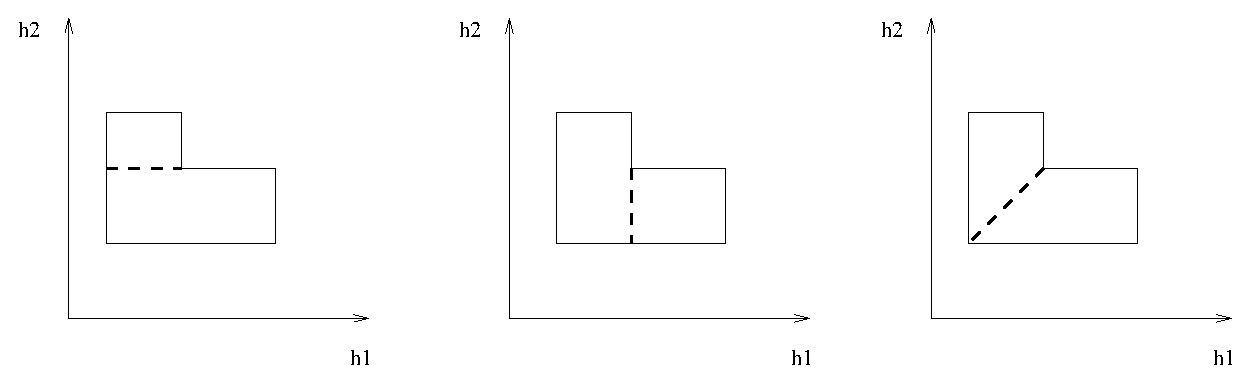
\includegraphics[width=\linewidth]{METHODS/decomp.eps}
\end{center}
\caption{Convex decompositions of a non-convex polyhedron\label{fig:decomp}}
\end{figure}
The lack of a canonical form militates against the efficient testing of
inclusion and equality. It is also difficult to check whether
the union of two or more polyhedra is in fact convex, and so could be
represented using a single DBM in order to reduce storage requirements.
\end{paragraph}

\subsection{Implementing constraint solving}
\subsubsection{Avoiding non-convex polyhedra}
In the previous section, we have seen a number of pragmatic reasons
for avoiding the use of non-convex polyhedra in implementing a
constraint-solving approach to the reachability problem. This has motivated
the investigation of methods which rely exclusively on convex polyhedra.
Recall that the reachability problem can be solved by computing the limit
of the sequence $\Z_0, \Z_1,\ldots$, where
\begin{eqnarray*}
\Z_0 & = & \{(\tgloc,\clkcond)\} \\ 
\Z_{i+1} & = & \{(\tgloc',\suc{\tgedge}{}(\clkcond)) |
                  (\tgloc,\clkcond) \in \Z_i \land 
                  \tgedge = (\tgloc,\tgguard_\tgedge,a,\someclks,\tgloc') \in 
                  \tgedges\} \uplus \\
         &   & \{(\tgloc,\suc{\tau}{\tgloc}(\clkcond)) | (\tgloc,\clkcond) \in
                  \Z_i\}  
\end{eqnarray*} 
It has been shown already that $\suc{\tau}{}$ and $\suc{\tgedge}{}$
preserve convexity. However, $\uplus$ can give
rise to non-convex polyhedra, because of the union of clock zones
which is implicit in its definition. This union can be
avoided simply by replacing it with a convex hull. In order to do this,
we redefine $\clkcond_\tgloc^\Z$, so that, for a set of
symbolic states $\Z$, $\chset{\clkcond_\tgloc^\Z} =
\bigsqcup\{\clkcond | (\tgloc,\clkcond) \in \Z\}$. If we modify the definitions
of $\unite$ and $\uplus$ to make use of this new definition, then all
operations required in computing $\Z_0, \Z_1, \ldots$, preserve the
convexity of polyhedra and so every clock constraint can be
represented by a single DBM, with all of the efficiency gains which
that implies. This approach has been adopted directly by
Balarin~\cite{bal:96} who combines it with a representation of the
complete state space using BDDs. The main problem with this method is
that the convex hull gives only an (over-)approximation of the set of
clock valuations associated with any location, and so, while the set of
reachable states is clearly included in $\Z=\lim_{i \geq 0}\Z_i$, it is clear that $\Z$ may also include states 
which are not in fact reachable. Moreover, the approximation errors
accumulate over the sequence $\Z_0, \Z_1,\ldots$. The consequence of
this is that the verification problem runs the risk of being answered
by a `false negative': i.e.,  we may be told that a specification is
not satisfied because a violating state is reachable, when, in fact
such a state occurs only among those `extra' states added by the
approximation.  Wong-Toi~\cite{wt:95} proposes a solution to this
problem in which a succession of over- and under-approximations is
computed. If a violating state is reachable in an under-approximation,
then the specification is not satisfied. If no violating state is 
reachable in an over-approximation, then the specification is
satisfied. An increasingly accurate sequence of approximations is
computed until the verification problem can be answered in this
way. However, in some cases, it may be necessary to compute an
approximation which captures the set of reachable states exactly,
before the verification problem can be answered -- this is less
efficient than a direct computation of the exact set of reachable
states. An alternative approach, which avoids the use of non-convex polyhedra
and also avoids the use of approximations, is considered below.

\subsubsection{Simulation Graph} \label{sec:mscsimgraph}
In this section we consider a construction, the \emph{simulation
graph}~\cite{oli:94,dt:98}, which has appeared often in the literature
of dense-time verification under a variety of names, including:
\emph{set-graph}~\cite{acd:92,wt:95},
\emph{zone automaton}~\cite{ad:96,ak:95} and 
\emph{symbolic semantics}~\cite{lpy:95,pet:99}. We first give details of the
construction and then consider the advantages and disadvantages of its
use.

\begin{definition}[Simulation Graph]\label{def:mscsimgraph}
Let $\AA = (\tglocs,\tgiloc,\Actions,\tgclks,\tgedges,\tginv)$ be a
TA. Let $c$ be a constant at least as great as $\cmax(\AA)$. The
\emph{simulation graph} of $\AA$ with respect to $c$, starting at the
symbolic state $\z_0 = (\tgloc_0,\vexcond_0)$, is denoted
$\SG(\AA,c,\z_0)$, and is given by $(\sgstates, \sginit, \Actions,
\goesSG{})$, where $\sgstates \subseteq \tglocs \cross \ClockZones$ and $\goesSG{} \subseteq \sgstates \cross \Actions \cross \sgstates$ are the smallest 
sets satisfying:
\begin{enumerate}
\item $\sginit = (\tgloc_0, \suc{\tau}{\tgloc_0}(\vexcond_0)) \in \sgstates$ 
\item for every $\z = (\tgloc,\vexcond) \in \sgstates$  and for every $\tgedge = (\tgloc, \vexcond_\tgedge, a, \someclks, \tgloc') \in \tgedges$, if $\vexcond' = \close{c}{\suc{\tau}{\tgloc'}(\suc{\tgedge}{}(\vexcond))} \neq \emptyset$,
then $\z' = (\tgloc',\vexcond') \in \sgstates$ and $\z \goesSG{a} \z'$
\qed
\end{enumerate}
\end{definition}

\begin{notation}
The simulation graph of $\AA$ with respect to $c$, starting
at the initial state $(\tgiloc,\cczero)$, is denoted simply by $\SG(\AA,c)$,
and $\SG(\AA)$ denotes $\SG(\AA,\cmax(\AA))$.
\end{notation}

Intuitively, a simulation graph of $\AA$ is constructed by starting
with a given symbolic state, and then allowing time to pass -- rule 1,
above; we then consider all the edges of $\AA$ and look for any which
can be taken from a node already in the graph; any possible edge
transition is taken and time allowed to pass again, the successor node
being added to the graph -- rule 2, above; $c$-closure is used to
ensure that the graph is finite; this process continues until all
possible nodes and edges have been added to the graph. 

Let $\AA = (\tglocs,\tgiloc,\Actions,\clocks,\tgedges,\tginv)$ be a TA
with $\TSys{\AA} = (\States,\Init,\Labels,\TRel)$. Let $c \geq
\cmax(\AA)$ and $\z$ a symbolic state. We now state the two key
properties of the simulation graph $\SG(\AA,c,\z) =
(\sgstates,\sginit,\Actions,\goesSG{})$.
\begin{proposition}
$\SG(\AA,c,\z)$ is finite.
\end{proposition}
\begin{proof}
This follows immediately from the fact that the locations and edges of
any TA are finite sets together with proposition~\ref{prop:cclosure}(4).
\end{proof}

\begin{proposition}[Correctness of simulation graph]\label{prop:simgraph} 
Assume, without loss of generality, that $\z$ is the symbolic state
$(\tgloc_0,\vexcond_0)$, where $\vexcond_0$ denotes the convex
$\clocks$-polyhedron which contains the single point $\clkvl_0$. Then,
\begin{itemize}
\item (Soundness) whenever $(\tgloc_0,\vexcond_0) \ngoesSG{\star} 
      (\tgloc_f,\vexcond_f)$ then $(\tgloc_0,\clkvl_0) \ngoes{\star}
      (\tgloc_f,\clkvl_f)$, for all $\clkvl_f \in \vexcond_f$;
\item (Completeness) whenever $(\tgloc_0,\clkvl_0) \ngoes{\star}
      (\tgloc_f,\clkvl_f)$ then $(\tgloc_0,\vexcond_0) \ngoesSG{\star}
      (\tgloc_f,\vexcond_f)$ for some $\vexcond_f$ such that 
      $\clkvl_f \in \vexcond_f$. 
\end{itemize}
\end{proposition}
\begin{proof}
Straightforward adaptation of theorem 4.1 in Pettersson~\cite{pet:99}
\end{proof}

It is clear from Proposition~\ref{prop:simgraph} that the reachability
problem can be solved by searching the simulation graph: in order to
determine if $(\tgloc',\clkvl')$ is reachable from $(\tgloc,\clkvl)$
in the transition system of $\AA$, it suffices to construct the
simulation graph $\SG(\AA,\cmax(\AA),\z)$ where
$\z = (\tgloc,\{\clkvl\})$; if there
is a node $(\tgloc'',\vexcond'')$ such that $\tgloc' = \tgloc''$ and
$\clkvl' \in \vexcond''$ then the answer is `yes', otherwise the
answer is `no'. Figure~\ref{fig:simgraphreach} outlines an algorithm
which implements this approach.
\begin{figure}
\begin{center}
\small
\NumberProgramstrue
\begin{programbox}
\INPUT
\AA=(\tglocs,\tgiloc,\Actions,\clocks,\tgedges,\tginv), c = \cmax(\AA),
\text{ initial state } (\tgloc,\clkvl), \text{ final state } (\tgloc',\clkvl')
\ENDINPUT
\BEGIN 
|VISITED| := \{(\tgloc, \{\clkvl\})\};
|WAITING| := \{(\tgloc, \{\clkvl\})\};
\WHILE |WAITING| \neq \emptyset \DO
    \text{remove some } (\tgloc'',\vexcond'') \text{ from }  |WAITING|
    \IF (\tgloc' = \tgloc'') \land (\clkvl' \in \vexcond'') 
    \THEN \RETURN \text{ `yes' }
    \ELSE 
      |succ| := \{(\tgloc_s,\vexcond_s) \vbar \tgedge = (\tgloc'',\_,\_,\_,\tgloc_s) \in \tgedges \land 
\t3 \vexcond_s = \close{c}{\suc{\tau}{\tgloc_s}(\suc{\tgedge}{}(\vexcond''))} \neq \emptyset\};
      \FOREACH (\tgloc_s,\vexcond_s) \in |succ| \DO
        \IF (\tgloc_s,\vexcond_s) \notin |VISITED|  
          \text{add } (\tgloc_s,\vexcond_s)\ \text{ to } |VISITED|;
          \text{add } (\tgloc_s,\vexcond_s)\ \text{ to } |WAITING|
        \FI
      \OD  
    \FI
\OD;
\RETURN \text{ `no' }
\END
\end{programbox}
\end{center}
\caption{An algorithm for reachability based on the simulation graph \label{fig:simgraphreach}}
\end{figure}

There are several reasons why reachability analysis based on the simulation
graph has been applied successfully:
\begin{itemize}
\item Only convex polyhedra are needed in the implementation of the algorithm.
  We have already seen that there are efficient algorithms for manipulating
  the DBM representation of convex polyhedra which ensures that the 
  membership test at line~9, the generation of successors at lines~12--13,
  the test for emptiness at line~13 and the implicit equality test at line~15
  can all be computed effectively.
\item The reachability test is performed `on-the-fly', i.e., it is not 
  necessary to generate explicitly the complete product automaton of
  several TA, nor is it necessary to generate the full state space,
  before checking whether or not a particular state is reachable. The
  test (at line~9) can be performed as the state space is constructed,
  and, indeed, in many cases the algorithm will terminate when only a
  small fraction of the total number of states has been generated.
\item A diagnostic trail can be provided based on the contents
  of $WAITING$, assuming a stack implementation. In practice, this is
  of great assistance to the user in the modification of an
  incorrect system.
\item Although the theoretical bound on the size of the simulation
  graph is exponential in the number of clock regions~\cite{acd:92},
  in practice, far fewer states are generated than in region graph
  algorithms -- sensitivity to the size of constants in clock
  constraints is alleviated.
\end{itemize}

\subsubsection{More heuristics}
The size of the set $VISITED$ of stored states can be reduced by employing
two further heuristics, one of which preserves reachability exactly and
the other of which preserves it conservatively. 
\begin{itemize}
\item \label{par:mscinclusion} 
  \emph{Inclusion abstraction} is based on the idea that for two
  symbolic states $\z_1$ and $\z_2$ such that $\z_1 \subseteq \z_2$,
  $\z_1$ need not be explored, since any state in $\z_1$ also belongs
  to $\z_2$, and any successor of $\z_1$ is also a successor of
  $\z_2$. The implementation of this idea simply involves a
  modification of the test at line 15 from $(\tgloc_s,\vexcond_s)
  \notin VISITED$ to $\lnot\exists \vexcond \in \ClockZones \such
  (\tgloc_s,\vexcond) \in VISITED \land \vexcond_s \subseteq
  \vexcond$. The effect of this is that instead of checking that a
  successor state is not already in the set of visited states, we
  check that there is no visited state which `covers' the successor
  state, in the sense of having the same control location and being
  associated with a set of clock valuations which includes all those
  of the successor. Clearly, this modification may reduce the number
  of symbolic states which are stored, while ensuring that all, and
  only, reachable states are considered. This technique is used in the
  tool UPPAAL~\cite{lpy:97} and in later versions of
  KRONOS~\cite{bdm:98}. A proof of correctness can be found
  in~\cite{dt:98,tri:98}.
\item \emph{Convex hull abstraction} implements the proposal mentioned
  above, in the section on avoiding non-convex polyhedra. Once again,
  the idea is to tolerate an over-approximation of the set of
  reachable states with the compensation that it is necessary to keep
  only a single symbolic state $(\tgloc,\vexcond)$ for each control
  location $\tgloc$. This can be implemented by replacing lines 15--18
  with the following:
\begin{center}
\small
\begin{programbox}
\IF \exists \vexcond \in \ClockZones \such (\tgloc_s,\vexcond) \in |VISITED|
   \THEN
  \IF \vexcond_s \not\subseteq \vexcond 
  \THEN
    \text{add } (\tgloc_s,\vexcond \hull \vexcond_s) \text{ to } |VISITED|
    \text{add } (\tgloc_s,\vexcond \hull \vexcond_s) \text{ to } |WAITING|
  \FI
\ELSE
    \text{add } (\tgloc_s,\vexcond_s) \text{ to } |VISITED|
    \text{add } (\tgloc_s,\vexcond_s) \text{ to } |WAITING|
\FI  
\end{programbox}
\end{center}
The advantages and disadvantages of this approach have been discussed already.
\end{itemize}

\subsection{Other attacks on state space explosion \label{ss:mscstateexplosion}}
In addition to the symbolic constraint solving algorithms of the
previous section, there are several other techniques which have been
applied to the problem of state space explosion in the analysis of
timed systems.  It is outside the scope of this dissertation to give a
detailed survey of the literature; instead, we briefly review some of
the most significant ideas.

\subsubsection{Large grain partitions} 
As we have seen, the primary objective of any verification algorithm
for TA, is to identify a finite partitioning of the infinite space of
clock valuations, where the partitioning respects the transition
relation. Although the region graph satisfies this requirement, it
produces a very fine partitioning with a large number of classes, and
so leads to algorithms which often require more computational
resources (memory and time) than are available. An interesting
question is whether or not it is possible to construct a partitioning
with the \emph{smallest number of classes} needed to solve a given
verification problem. This question can be answered positively in the
case of timed bisimulation equivalence and model checking. 

The problem of constructing the quotient of a LTS with respect to an
equivalence relation is well-known in the setting of untimed systems,
and generic algorithms exist to solve the problem~\cite{bfh:92,ly:92}.
These algorithms have been adapted to TA in~\cite{acd:92,ach:92},
where it is shown how to simultaneously generate and minimise the
reachable sub-LTS of a TA.  Tripakis and Yovine~\cite{ty:96} have
shown how such minimisation can be performed more efficiently by
adapting the idea from~\cite{yl:93} of avoiding the costly operation
of set complementation. Once constructed, the minimal model of a TA
may be reduced still further with respect to untimed abstractions, and
then checked for equivalence with an untimed specification automaton
using a tool such as CADP~\cite{fgk:96}.  

A similar use of large-grained partitions is made by Sokolsky and
Smolka~\cite{ss:95,sok:96} to solve the full model-checking problem
for a timed modal $\mu$-calculus. In their approach, partition
refinement is applied to a structure which models the `product' of the
symbolic state space and a graph representation of the property
specification; their algorithm strives to construct the coarsest
possible partitioning which allows the validity of the specification
to be decided. Recent work by Lutje-Spelberg et al.~\cite{lta:98} seeks to
improve on this approach by using a more compact representation
of the set of regions which a partition comprises.

\subsubsection{Partial Order Reduction}
In asynchronous system models, state space explosion is due partly to
the modelling of concurrency by interleaving, whereby the simultaneous
occurrence of two or more events is represented by a set of executions
which contains all possible orderings of those events. Partial order
reduction exploits the observation that it is not always necessary to
consider the whole set of such executions, but rather to consider only
one representative from each of the classes of `equivalent'
executions~\cite{god:96,pel:92,val:93}. The application of partial
order techniques in tools for the analysis of untimed systems has
demonstrated significant state space
reduction~\cite{hol:96,hp:94}. However, similar success has not (yet)
been demonstrated for real-time systems. A major difficulty seems to
be that the independence of system components is reduced by their need
to synchronise with each other in respect of the passage of
time~\cite{ys:96,pag:96,pag:97}. Bengtsson et al.~\cite{bjl:98} have
recently proposed the use of `local' clocks in TA, which usually
advance independently and are synchronised only when there is a need
for communication.  Dams et al.~\cite{dgk:98} suggest a different
approach which incorporates a generalised notion of independence, called
`covering'. Both of these approaches are intended to allow a greater
potential for independent behaviour and so to give a coarser
partitioning of the set of executions into `equivalent' classes. So
far as we know, there are as yet no successful implementations of
partial order reduction methods for dense real-time systems.

\subsubsection{Abstraction} 
All modelling and analysis relies upon abstracting details from the
system under investigation, while keeping what is necessary to
preserve the properties of interest. An extreme example of abstraction
can be seen in approaches which abstract all details of data values
from their models, leaving only control information. Less extreme
methods of property-preserving abstraction, set within the framework
of \emph{abstract interpretation}~\cite{cc:77}, have been proposed
in~\cite{cgl:94,lgs:95,sbl:99}. Application to the verification of LTL
properties is discussed in~\cite{kp:98}. In the case of timed systems,
the possibility of abstracting all timing information initially,
adding it only when it is known to be needed to demonstrate a given
property, has been investigated in~\cite{aik:95}. A different approach
is adopted in~\cite{ty:96}, where timed models are constructed
initially and then reduced according to a time-abstracting
bisimulation. Daws and Tripakis have placed a number of standard
techniques for reducing the size of timed systems within the framework
of property-preserving abstractions~\cite{dt:98}. The problem of
demonstrating that a timed system model is a correct abstraction of a
more concrete system is considered in~\cite{tak:96}. A combination of
abstraction with other techniques is the norm. When used in conjunction
with modular reasoning and/or theorem proving, it can extend the scope
of model checking to systems with infinite state
spaces~\cite{aab:99,df:95,rss:95,ss:99}.

\subsubsection{On-the-fly techniques}
A system model comprising a set of concurrent tasks exhibits state
explosion when the product space is constructed. On-the-fly methods
combat state explosion by solving a problem \emph{during} the
construction of the product space, rather than \emph{after} it. This
means that the full product space may not need to be constructed at
all, and so state explosion can be avoided. This technique has been
applied successfully in solving reachability problems~\cite{jj:89},
computing behavioural equivalences and preorders~\cite{fm:91},
checking temporal logic properties~\cite{gpv:95,vw:86} and minimising
state graphs~\cite{bfh:92}. Extension of the technique to the solution
of similar problems in timed systems has been considered
in~\cite{bty:97,hkv:96,ty:96}. On-the-fly methods are most useful when
debugging a system, i.e.  when checking properties which turn out not
to hold. It is difficult to avoid considering all reachable states
when checking a true property.

\subsubsection{Symbolic methods}
The model checking approach was given a big boost by the work of
McMillan in the late eighties~\cite{mcm:92}. He discovered that
regularly structured state spaces, such as those derived from models
of hardware components or communication protocols, can be represented
very compactly using binary decision diagrams (BDDs)~\cite{bry:86}.
The operations needed for model checking can be adapted to work with
sets of states, represented as BDDs, rather than individual states.
Using this technique, it is possible to verify systems having more
than $10^{20}$ states~\cite{bcm:92}. So far, the benefits of such
symbolic techniques have not been realised completely in the analysis
of timed systems. We consider this problem in more detail in
Chapter~\ref{chap:sggen}.
   
\subsubsection{Modular/Compositional Verification}
We have seen that many systems are implemented and modelled as the
composition of several components. Yet another approach to avoiding
the construction of the product of the component state spaces is to
decompose a global system property into a number of local properties
of one or more components, and then to prove that, if the local
properties are satisfied, the global property is satisfied also. The
intention here is to transform a single, large verification problem
into several smaller problems~\cite{gl:94}.  In proving a local
property, it is often convenient to \emph{assume} that the environment
behaves in a certain manner; it is then necessary for the other system
components to \emph{guarantee} this behaviour. The assume/guarantee
paradigm is discussed in~\cite{hqr:98}.  The task of decomposing a
problem can require significant insight and often defies automation.
An approach which can be automated involves the computation of a
quotient property with respect to some component which is then removed
from the system model, such that proving the quotient property in the
reduced model is equivalent to proving the original property in the
original model.  Iteration of this technique allows a property to
verified automatically without having to construct the product state
space. This approach has been applied to timed systems~\cite{kll:97}
and implemented in the model checker CMC~\cite{ll:98}. A different
approach to automating compositional analysis is introduced
in~\cite{lab:98}. In this approach, backwards reachability analysis is
performed using only those components which are required to determine
the property of interest. Dependency analysis is used to determine
which components are relevant. The technique has been applied
successfully to embedded systems but its scope has not yet been
extended to include timed systems.

\subsubsection{Clock reductions}
The state explosion problem in timed systems is compounded by the need
to take account of clock values~\cite{ad:94}. The most significant
attack on this aspect of the problem is the work of Daws and
Yovine~\cite{dy:96} which shows two methods for reducing the number of
clocks needed in a TA:
\begin{itemize}
\item \emph{Clock activity reduction} relies on identifying for each TA 
location those clocks which do not affect the behaviour of the TA before
they are reset. Such clocks are said to be \emph{inactive}; the
other clocks are said to be \emph{active}. It is only necessary to record 
the values of the active clocks in each location, so reducing the memory
requirements for a set of timed states.
\item \emph{Clock equality reduction} is achieved by identifying those
clocks whose values are equal in all locations. Such a set of equal-valued
clocks can be replaced by a single clock. 
\end{itemize}
Another technique, with a similar purpose, has been introduced
in~\cite{llp:97}. The aim here is to replace a DBM $\M$ with a minimal
set of clock constraints whose solution set is the same as $\M$'s.  An
algorithm is given which computes a minimal set of constraints for any
DBM.  Memory requirements are reduced by storing this minimal set
rather than the full DBM.

\subsection{Tools}
There is now a large number of well-developed computer programs which
implement automatic verification of finite state systems
(see~\cite{ck:96} for a survey). Here we concentrate exclusively on
those tools which have been shown to be effective in the analysis of
dense real-time systems, and which implement the techniques mentioned
earlier in this section.
  
\begin{description}
\item[COSPAN] has been developed at AT\&T and applied
to a number of industrial-scale examples, being the basis of the
commercial tool {\sf FormalCheck}. It is based on the theory of
$\omega$-automata~\cite{kur:94} and allows both enumerative and BDD-based
search~\cite{tbk:95} and homomorphic reductions~\cite{tak:96}. Real-time
verification can be performed using either the region graph or the
simulation graph~\cite{ak:95} and timing constraints can be checked
incrementally~\cite{aik:95}.
\item[HYTECH] is a symbolic model checker for linear hybrid 
automata~\cite{hhw:97}, which may be seen as generalising TA by
allowing the use of continuous variables to model other aspects of
system state than time, e.g., temperature or pressure. A system is
described as a set of coordinating linear hybrid automata and a
symbolic fixpoint computation is used to check the validity of a
specification given as an expression in a branching real-time logic
which extends TCTL~\cite{ach:95}. The tool has been used to verify a
number of small examples~\cite{ahh:96}, including the Philips audio
transmission protocol~\cite{hw:95}. A key feature of HYTECH is its
ability to perform parametric analysis, i.e., to determine the values
of design parameters for which a linear hybrid automaton satisfies a
temporal logic requirement.
\item[KRONOS] was developed originally by Sergio Yovine 
to implement the model-checking of TA with respect to TCTL
specifications using the symbolic method proposed
in~\cite{hnsy:94}. It has since been extended with procedures for:
on-the-fly checking of TBA emptiness~\cite{bty:97}, generation of
minimal models by time-abstracting bisimulation~\cite{ty:96},
automatic reduction of the number of clock
variables~\cite{daw:98a,dy:96}, inclusion and convex hull
abstraction~\cite{dt:98}, and symbolic state space representation
using BDDs~\cite{bmp:97}.  The PhD dissertations of
Tripakis~\cite{tri:98} and Daws~\cite{daw:98} give detailed
descriptions of the most recent technical advances which are
implemented in the current version of the tool. The effectiveness of
KRONOS has been demonstrated through its application to several case
studies, including: the Philips audio transmission
protocol~\cite{dy:95}, the CNET protocol~\cite{ty:98} and the STARI
chip~\cite{bmp:97}.
\item[UPPAAL] allows the checking of networks of TA based on reachability
analysis of the simulation graph as described earlier. The underlying
principles of this approach were described in~\cite{ypd:94}. The
property specification language allows the expression of safety
properties, including bounded response, and also simple liveness
properties of the form $\ealways{} p$ and $\aeventually{} p$,
where $p$ is a `locally' checkable state property. The tool also
reports all deadlocked states (i.e., states where no discrete
transition will be possible in the future) encountered during a
verification. Since its first release in 1995~\cite{bll:95}, UPPAAL
has been improved by the introduction of a more efficient
representation of clock constraints, a new termination algorithm which
requires the storage of fewer visited states~\cite{llp:97}, and an
improved hash table implementation of the set of visited
states~\cite{bll:98}. An important feature of UPPAAL, from the point
of view of usability, is a graphical interface which integrates the
various features of the tool, such as system description, property
specification, simulation and verification. UPPAAL is now sufficiently
mature to have been used in a number of industrial case studies,
including the analysis of communication protocols such as the Bang \&
Olufsen audio/video protocol~\cite{hsl:97}, the Bounded Retransmission
protocol~\cite{dkr:97}, the Dacapo startup protocol~\cite{lp:97} and a
lip synchronisation algorithm for the transmission of multimedia
data~\cite{bfk:98}. It has also been used in a collaborative project
with the automotive industry to assist in the design of a gear
controller~\cite{lpy:98}.
\end{description}
Other interesting approaches for which tools exist, although perhaps
less well-developed and case-tested than those mentioned above,
include: VERITI~\cite{wt:95} which implements Wong-Toi's method based
on successive over- and under-approximation; RT-SPIN~\cite{tc:96}
which extends ProMela, the language of the model-checker
SPIN~\cite{hol:96}, with simple time guards and performs
constraint-based reachability analysis on the derived TA;
SGM~\cite{hw:98} which provides an environment in which it is possible
to experiment with different combinations of several state graph
manipulators~\cite{wh:98,wh:98b} in order to reduce the size of the
state space; PMC~\cite{lta:98} which implements the partition
refinement algorithm of Lutje-Spelberg et al.; and CMC~\cite{ll:98} which
implements an improved version of the compositional approach to model
checking which was first introduced in~\cite{ll:95}.

\section{Conclusions}\label{sec:mscconc}
This chapter has reviewed an approach to the formal modelling and
analysis of real-time systems. Systems are modelled as labelled timed
transition systems over a dense time domain. We have considered the
expression of such models using timed process algebra and timed
automata. Specifications are given either as expressions in a timed
temporal logic such as TCTL, or as specification automata. Analysis
techniques are based upon exhaustive state space search, where the
major difficulty is the state explosion problem. We have discussed in
detail approaches to this problem in which sets of clock valuations are
represented as linear constraints, implemented efficiently using DBMs.
These languages and methods are the foundation for the work presented in  
the rest of the dissertation.

This review has necessarily omitted consideration of many other
approaches to the modelling and analysis of timed systems, which have
appeared in the literature in recent years. We take a small step to
fill this gap by briefly mentioning some of them now. 

There is a large Petri net community which has established many
theoretical results and practical techniques for modelling and analysis. In
this context, a variety of timed Petri nets have been suggested for
use with timed systems~\cite{bd:91,rok:93,sif:77}.

Graphical modelling languages are of interest since many designers
find a visual syntax `intuitively' clear. Hierarchical structures are
needed in order to manage the size of the diagrams for all but the
simplest systems. Statecharts~\cite{har:87} allow such a hierarchical
representation of untimed state transition
models. Modecharts~\cite{jlm:88,jm:87,ymw:93} extend this approach
with explicit timing constraints; another timed Statechart extension,
which can be used for modelling hybrid systems also, is given
in~\cite{kp:92}.

Lynch and Vaandrager have introduced timed I/O automata, which offer
a similar model of timed systems to the timed automata discussed in
this chapter; rather than verification via model-checking, they
propose refinement and simulation proof techniques~\cite{lv:96}.

Cardell-Oliver~\cite{car:92} proposes the use of higher order logic
both to model the behaviour of a system and its environment, and also
to specify requirements. The task of proving that the combined system
and environment satisfy the requirements is supported by the use of a
mechanical theorem prover. Hooman~\cite{hoo:91,hoo:96} offers a
related assertional style of modelling and specification using
extended Hoare triples~\cite{hoa:69}. Duration
Calculus~\cite{chr:91,liu:96} is yet another approach in which
modelling and verification is conducted within a single logical
framework.

Validation of real-time systems by means of formally constructed test
suites is considered in~\cite{cg:98,svd:97}.








